% ============================================================================
% Segmented execution — JSA submission (VSI: Security and Efficiency for
% LLM-Based Edge Intelligence). Free-format (Your Paper Your Way) first
% submission; elsarticle conversion at revision.
% Build: pdflatex + bibtex (IEEEtran.bst).
% ============================================================================
\documentclass[journal]{IEEEtran}
\usepackage{amsmath,amssymb,amsthm}
\usepackage{graphicx}
\usepackage{booktabs}
\usepackage[colorlinks=true,linkcolor=blue,citecolor=blue,urlcolor=blue]{hyperref}
\newtheorem{proposition}{Proposition}
\newtheorem{theorem}{Theorem}

\begin{document}

\title{Segmented Execution of Large Language Models:\\
Sequential Training and Inference on Resource-Constrained Devices}

\author{%
Sadegh~Keshtkar,
Saad~Ahmad,
Michael~Bidollahkhani,
and~Julian~Kunkel%
\thanks{S.~Keshtkar, S.~Ahmad, M.~Bidollahkhani, and J.~Kunkel are with the
Institute of Computer Science, University of G\"ottingen, 37077 G\"ottingen,
Germany. M.~Bidollahkhani and J.~Kunkel are also with GWDG, 37077
G\"ottingen, Germany. Corresponding author: Sadegh Keshtkar (e-mail:
keshtkar.sadegh@gmail.com).}%
\thanks{This work was supported by the Federal Ministry of Education and
Research (BMBF), Germany, under the AI service center KISSKI (grant nos.\
01IS22093A and 01IS22093B).}%
}

\markboth{Preprint --- submitted to the Journal of Systems Architecture}{Keshtkar \MakeLowercase{\textit{et al.}}: Segmented Execution of Large Language Models}

\maketitle

\begin{abstract}
Devices with limited memory---edge nodes, commodity CPUs, single mid-range
accelerators---are widely considered unable to train or even load large
language models (LLMs). We argue this limit is set by framework scheduling
rather than by the computation, and present segmented execution: a GPT
decoder is partitioned along four cut planes (attention head groups,
feed-forward hidden units, embedding width, and vocabulary slices) and
executed sequentially---one small segment computing at a time, and, in the
streamed modes, at most one segment resident, while everything else waits
in host memory or on disk. A small set of dials (recomputation, weight
streaming, dropout, key--value caching, and the update schedule) defines
operating modes that trade memory for time, and every mode is verified to
compute the same model: bit-deterministic on CPU, with identical
predictions across all engines including a PyTorch-free ONNX runtime---the
data never has to leave the device that owns it. A 0.84-billion-parameter
decoder trains in 1.1~GB of device memory, 23 times below full-model
training and 20 times below the DeepSpeed ZeRO-Offload floor; a
6.9-billion-parameter model, whose full-model training aborts even on a
94~GB accelerator, trains on a CPU-only node in 9.3~GB of RAM, on a single
40~GB accelerator, or in 2.6~GB when streamed; and the smallest serving
mode answers queries in 401~MB without a GPU or a training framework. The
price is time---$5.4\times$ full-model step time at half its memory to
$30\times$ at the memory floor---captured in analytic memory and time laws
validated by a pre-registered prediction on a held-out configuration.
Every headline mode is further validated over hundreds to thousands of
consecutive training steps and serving requests: device memory stationary
to the byte on GPU and bounded on CPU, with long-run latencies down to
31~ms per token for resident 0.84B serving.
\end{abstract}

\begin{IEEEkeywords}
Large language models, on-device learning, edge intelligence,
memory-efficient training, offloading, runtime systems.
\end{IEEEkeywords}

% ============================================================================
\section{Introduction}\label{sec:intro}
% ============================================================================
\IEEEPARstart{T}{he} capability frontier of language models has advanced in
lockstep with the memory of the hardware that trains and serves them.
Contemporary practice assumes a data-center substrate of tens to hundreds of
gigabytes of high-bandwidth memory, with frameworks tuned to keep it
saturated, under which a simple rule holds: \emph{if the model, its optimizer
state, and its activation graph do not fit, you cannot train it on that
device.}

A growing class of settings inverts these assumptions. Edge devices, IoT
endpoints, and mobile phones are defined by tight, fixed memory; their compute
is often idle, battery- or thermally limited, and latency-tolerant or entirely
offline. More fundamentally, much of the data that would most benefit from
adaptation is private and non-exportable (health records, personal messages,
on-device sensor streams, regulated enterprise data), so the only compliant
place to train or fine-tune on it is the device that holds it---and the
natural way to learn \emph{across} such data holders is federated
learning~\cite{mcmahan2017federated}, which presupposes exactly what today's
frameworks deny: that each resource-constrained participant can run training
locally. This paper builds that missing substrate; the federated and
distributed instantiations on top of it are our declared next step
(Sec.~\ref{sec:limits}). Keeping training and inference on the device that
owns the data removes the network and server-side attack surface entirely:
no raw records, gradients, or activations ever cross a network boundary
(threats that require physical or privileged access to the device itself
are a separate matter; Sec.~\ref{sec:disc}). We note up
front that our mechanism is orthogonal to the edge community's default
lever, reduced precision: quantization and low-precision training shrink
every memory term by a constant factor~\cite{nadalini2023reduced,micikevicius2018mixed},
whereas segmentation bounds which terms must coexist at all---and the two
compose \emph{productively}: quantized segments are smaller, so a fixed
memory budget affords a coarser partition, and coarser partitions are the
faster end of the granularity dial (Sec.~\ref{sec:gran}); quantization
inside segmented execution therefore buys back time as well as memory. All
results here are deliberately full-precision fp32 so that exactness can be
verified end to end. For these
settings the binding constraint is \emph{memory}, not FLOPs, and the question
is not ``how do we make the model fit the machine?'' but ``how do we make the
\emph{computation} fit a memory budget we are given?'' This memory-bound
character is not unique to the edge: even large-batch data-center inference is
now found to be bottlenecked by memory and DRAM bandwidth rather than
compute~\cite{tazi2025memorygap}.

This paper takes the position that \emph{memory is a budget, not a
requirement}. The peak memory of a standard training step decomposes into
parameters, gradients, optimizer state, a retained activation graph, and
framework runtime overhead, and every one of these terms is a design choice in
service of speed when memory is plentiful, not a mathematical necessity. We
therefore execute the model \emph{one segment at a time}. The decoder is
partitioned along the same four axes that tensor
parallelism~\cite{shoeybi2019megatron} cuts across devices---attention head
groups, feed-forward hidden units, embedding width, and vocabulary
slices---but where tensor parallelism multiplexes the partitions across
\emph{space} (one device per part, collectives joining them), segmented
execution multiplexes them across \emph{time}: one device visits the parts in
sequence, and the collectives degenerate into local concatenations and
accumulations. We refer to this duality as \emph{temporal tensor parallelism}.
An execution engine runs exactly one segment at a time; under weight
streaming it further guarantees that at most one segment is \emph{resident}
on the constrained device, every other segment, gradient, and optimizer
moment parked in a backing store (host memory behind a GPU, disk behind a
CPU), while the resident modes trade that memory floor for speed by keeping
all segment weights on the device. The
partition is a pure execution concern on an unchanged architecture, and we
verify that segmented training reproduces full-model training to
floating-point tolerance and matches its accuracy exactly at the prediction
level. \emph{The learning is invariant; only the memory schedule changes.}

Where prior single-device systems keep at least one full transformer
\emph{layer} resident~\cite{pudipeddi2020l2l,ren2021zerooffload,sun2022stronghold,fang2022patrickstar},
the residency floor here is one \emph{segment} of one layer. On top of the
partition, a small set of binary \emph{dials}---activation recomputation,
weight streaming, dropout, key--value caching at inference, and the optimizer
update schedule---defines a lattice of named \emph{operating modes}, in the
way ZeRO names its stages~\cite{rajbhandari2020zero}: a practitioner reads a
memory or time budget and selects a row. The modes span, on one 40~GB
accelerator for a 0.84B-parameter decoder, from 11.5~GB at $5.4\times$
full-model step time to 1.16~GB at $30\times$ (1.08~GB at $39\times$ with
the deferred update schedule); a fine partition reaches 890~MB. The same
dials govern inference, down to a 401~MB PyTorch-free serving mode.

\paragraph{Contributions.}
\begin{enumerate}
\item \textbf{Segmented execution as temporal tensor parallelism:} a
  four-axis partition of an unchanged GPT decoder executed one segment at
  a time---down to a one-resident-segment floor when streamed---with the
  reassembly identities stated as
  propositions and exactness across all operating modes established at the
  forward, gradient, optimizer-step, and prediction levels
  (Secs.~\ref{sec:design} and \ref{sec:exact}).
\item \textbf{A mode taxonomy instead of a technique zoo:} an always-on base
  of six memory bounds plus dials yields 12 training modes and 4 inference
  modes, each measured on GPU and CPU with device \emph{and} host memory,
  reported with its fastest and smallest representative at every model size
  and partition (Sec.~\ref{sec:eval}).
\item \textbf{Optimizer-in-backward at segment granularity:} fusing the
  parameter update into the backward pass~\cite{lv2024lomo} eliminates the
  separate optimizer sweep entirely (4.1~s${\to}$0.11~s per step on GPU,
  28~s${\to}$0.03~s on CPU), making the fastest resident mode $5.4\times$
  full-model step time and cutting streamed-mode time by 23\% and its host
  store by 4~GB (Sec.~\ref{sec:eval}).
\item \textbf{Capability results:} 0.84B trains in 1.08~GB (20$\times$ below
  the DeepSpeed ZeRO-Offload floor we measure); a 6.9B model whose full-model
  training aborts on a 94~GB H100 trains \emph{resident} on a single 40~GB
  A100 at 28.5~GB, moving the single-device wall past 6.9B
  (Sec.~\ref{sec:eval}).
\item \textbf{An exactness methodology with a falsification control:} the
  deviation of segmented from full-model execution is bounded \emph{below}
  the deviation of plain PyTorch from itself under a routine batch split, and
  all engines and modes, including the ONNX runtime, agree on every one of
  11{,}654 test predictions (Sec.~\ref{sec:exact}).
\item \textbf{An analytic cost model over size and partition,} fitted once
  on the measured grid (memory law within 8.7\% worst-case across five sizes
  and three partitions) and validated by a pre-registered prediction on a
  never-measured configuration, conservative by 7\% in time and 5\% in
  memory (Sec.~\ref{sec:model}).
\item \textbf{The framework-artifact argument:} a decomposition showing the
  residual time cost is dominated by schedulable data movement and
  per-segment dispatch, not by essential computation or link bandwidth---with
  the PyTorch-free runtime as direct evidence (Sec.~\ref{sec:disc}).
\end{enumerate}

% ============================================================================
\section{Background and Related Work}\label{sec:background}
% ============================================================================
\subsection{The Framework Memory Model}\label{sec:memmodel}
To argue that memory is a budget rather than a requirement, we separate what
the \emph{computation} needs from what the \emph{framework} takes. The peak
memory of a standard training step is, to first order,
\begin{equation*}
\begin{split}
\text{peak} \approx{}& \text{params} + \text{grads} + \text{opt\_state}\\
&+ \text{retained\_activations} + \text{runtime}.
\end{split}
\end{equation*}
For $P$ parameters in 32-bit with Adam the first three terms are $\approx
16P$ bytes, independent of batch or sequence length; the retained activation
graph scales with depth$\times$width$\times$batch$\times$sequence and
frequently dominates; the runtime term is the CUDA context ($\sim$0.5\,GB)
plus caching-allocator slack. Each exists for \emph{speed under abundant
memory}, not correctness. \emph{Eager execution with an autograd tape} keeps
all forward activations resident until backward so backpropagation is one
fast reverse sweep. The \emph{caching allocator} reserves large pools so
allocation leaves the critical path; reserved memory routinely exceeds live
memory. \emph{Kernels, fused attention, and the KV cache} favour large
resident operands and trade memory for speed. These choices target one
regime---\emph{memory is abundant, maximize FLOP/s}---and the field's
trajectory (larger HBM, faster interconnect, paged KV caches, deeper fusion)
entrenches it; resource-limited users are underserved by \emph{priority}, not
physics. Because every term is a scheduling choice, each has a memory-frugal
alternative: the activation graph can be \emph{recomputed}, parameters and
state can be \emph{streamed}, and logits and scores can be \emph{bounded}.
The rest of the paper makes these substitutions and measures their cost.

\subsection{Scaling Out vs.\ Scaling Down}
Most systems work on large-model training scales \emph{out}:
tensor~\cite{shoeybi2019megatron,narayanan2021megatron} and
pipeline~\cite{huang2019gpipe} parallelism and sharded data-parallel
training~\cite{rajbhandari2020zero,zhao2023fsdp} partition a model across
\emph{many} accelerators so that their aggregate memory suffices; 2D
tensor-parallel schemes additionally partition the hidden and embedding
width~\cite{wang2022tesseract}. This is complementary to, but the opposite
of, our goal: it lowers memory \emph{per device} only by adding devices,
whereas we lower the memory a \emph{single} device needs below a chosen
target. Mixed-precision training~\cite{micikevicius2018mixed} shrinks several
terms by a constant factor but leaves both the abundant-memory assumption and
the resident activation graph intact.

\subsection{Fitting a Model into Less Memory}
Closer to our aim are methods that reduce the memory a step needs.
\emph{Recomputation.} Activation checkpointing originates in reverse-mode
automatic differentiation~\cite{griewank2000revolve} and entered deep
learning as gradient checkpointing~\cite{chen2016training}, with
solver-optimal schedules~\cite{jain2020checkmate,shah2021monet}, selective
recomputation at scale~\cite{korthikanti2023selective}, and reversible
architectures~\cite{gomez2017reversible}; we take recomputation to its limit
(\emph{no} retained graph) and combine it with sub-layer streaming.
\emph{Swapping and offloading.} Out-of-core executions swap activations or
tensors between device and host~\cite{rhu2016vdnn,le2019tflms,huang2020swapadvisor,peng2020capuchin,wang2018superneurons};
ZeRO-Offload and ZeRO-Infinity stream optimizer state and parameters to CPU
and NVMe~\cite{ren2021zerooffload,rajbhandari2021zeroinfinity}; MemAscend
optimizes host-memory fragmentation and pinned buffers for SSD-offloaded
LLM fine-tuning on exactly the limited-resource hardware we
target~\cite{liaw2026memascend}, and recent planners co-optimize GPU and
CPU memory for fine-tuning under tight
budgets~\cite{ding2026heteropipeline,zhang2026memorysafe}.
\emph{Layer-granular streaming.} Layer-to-layer
execution~\cite{pudipeddi2020l2l}, working-window
offload~\cite{sun2022stronghold}, chunk-based heterogeneous memory
management~\cite{fang2022patrickstar}, and SSD-centric
fine-tuning~\cite{liao2025lohan} keep roughly one layer resident at a time
and reach tens to hundreds of billions of parameters on one accelerator.
\emph{Optimizer-memory reduction.} LOMO fuses the parameter update into the
backward pass so gradients are never materialized in
bulk~\cite{lv2024lomo,lv2024adalomo}; GaLore projects gradients and moments
to low rank~\cite{zhao2024galore}; factored and quantized
moments~\cite{shazeer2018adafactor,dettmers2022eightbit} and zeroth-order
updates~\cite{malladi2023mezo} shrink or eliminate optimizer state, the
latter approximately.
\emph{Memory-bounded inference.} Placement policies over GPU, CPU, and
disk~\cite{sheng2023flexgen}, flash-resident weights~\cite{alizadeh2024llmflash},
and layer-wise fetch~\cite{rajbhandari2021zeroinfinity} serve models beyond
device memory; the widely deployed llama.cpp
runtime~\cite{gerganov2023llamacpp} memory-maps quantized weights for
CPU-class inference; TPI-LLM pages tensor-parallel weight slices through
low-resource devices at inference time~\cite{li2025tpillm}; collaborative
serving distributes layers across peers~\cite{borzunov2023petals}.

\subsection{Memory-Efficient Kernels and Lossy Compression}
Fused attention computes exact attention without materializing the score
matrix~\cite{rabe2021selfattention,dao2022flashattention}; chunked and fused
cross-entropy never materializes the logit
matrix~\cite{milakov2018online,wijmans2025cce,hsu2024liger}; blockwise
formulations extend the same idea to the feed-forward
network~\cite{liu2023blockwise}. These exact kernels form part of our
always-on base. Quantization and low-rank adaptation
(LLM.int8()~\cite{dettmers2022llmint8}, GPTQ~\cite{frantar2022gptq},
LoRA/QLoRA~\cite{hu2022lora,dettmers2023qlora}) reduce memory by changing
\emph{what} is computed and are therefore lossy; they are orthogonal and
composable with our lossless partitioning.

\subsection{On-Device, Edge, and Private Computation}
On-device training under kilobytes to megabytes of
memory~\cite{lin2022ondevice} and federated learning~\cite{mcmahan2017federated}
are driven by the same constraints we target---fixed device memory and data
that cannot be exported---but typically assume small models or update only a
parameter subset. Lightweight inference runtimes such as ONNX Runtime execute
an exported graph without a training framework; we exploit this directly as
evidence that a share of what is called ``model memory'' is in fact runtime
overhead.

\subsection{Positioning}
Table~\ref{tab:landscape} situates this work among the closest systems, by
their own reported properties.
Every single-device system above has a residency floor of one transformer
layer (or the whole model). Our claim is that the floor can be pushed one
level lower, to one \emph{segment} of one layer, by applying the cut planes
of tensor parallelism~\cite{shoeybi2019megatron} temporally rather than
spatially---and that this can be done \emph{exactly}, with the deviation from
full-model execution bounded below the run-to-run deviation of the framework
itself. Where prior work ships an operating point or a solver-chosen
policy~\cite{sheng2023flexgen}, we characterize the whole configuration space
as a small lattice of named modes and validate an analytic cost model over
both model size and partition. Closest in spirit, concurrent work trains
federated clients block-wise in sequence to fit device
memory~\cite{wu2026blockwise}---at layer granularity and inside an FL
protocol; our four-axis sub-layer partition, exactness guarantee, and
mode taxonomy are the single-device substrate such systems presuppose.

\begin{table}[t]
\caption{The closest systems, by their reported properties. ``Trains'' =
full-parameter training/fine-tuning on the constrained device;
``sub-layer'' = residency floor below one transformer layer; ``verified
equivalence'' = published bit/roundoff-level identity with unmodified
full-model execution; ``framework-free serving'' = inference without the
training framework; ``lossless'' = no quantization/approximation required
by the method. ---~=~not reported.}
\label{tab:landscape}
\centering
\scriptsize
\setlength{\tabcolsep}{2.5pt}
\begin{tabular}{@{}lccccc@{}}
\toprule
System & Trains & Sub-layer & Verified equiv. & Fw.-free serving & Lossless \\
\midrule
ZeRO-Offload~\cite{ren2021zerooffload} & \checkmark & --- & --- & --- & \checkmark \\
PatrickStar~\cite{fang2022patrickstar} & \checkmark & --- & --- & --- & \checkmark \\
STRONGHOLD~\cite{sun2022stronghold} & \checkmark & --- & --- & --- & \checkmark \\
LoHan~\cite{liao2025lohan} & \checkmark & --- & --- & --- & \checkmark \\
MemAscend~\cite{liaw2026memascend} & \checkmark & --- & --- & --- & \checkmark \\
FlexGen~\cite{sheng2023flexgen} & --- & --- & --- & --- & --- \\
llama.cpp~\cite{gerganov2023llamacpp} & --- & --- & --- & \checkmark & --- \\
TPI-LLM~\cite{li2025tpillm} & --- & \checkmark & --- & --- & \checkmark \\
This work & \checkmark & \checkmark & \checkmark & \checkmark & \checkmark \\
\bottomrule
\end{tabular}
\end{table}

% ============================================================================
\section{Segmented Execution: Design}\label{sec:design}
% ============================================================================
\subsection{Partition and Reassembly Identities}\label{sec:partition}
The architecture is unchanged; segmentation is a pure execution concern, and
the union of segment weights reassembles the reference model exactly. A
configuration is written $E{\times}A{\times}M{\times}H$: the token and
position embeddings are split into $E$ slices along the model width
$d_\text{model}$; each attention block into $A$ head groups; each feed-forward
block into $M$ chunks along the hidden width $d_\text{ff}$; and the output
head into $H$ vocabulary slices. Layer norms, the attention output projection
$W_o$, and biases are shared parameters outside the partition. Exactness
rests on three algebraic identities.

\begin{proposition}[Concatenative reassembly]\label{prop:concat}
The embedding of a token is the concatenation over slices of the per-slice
embeddings, and multi-head attention output before $W_o$ is the concatenation
over head groups of the per-group attention outputs. Both hold \emph{bitwise}
in floating point: concatenation performs no arithmetic.
\end{proposition}

\begin{proposition}[Additive reassembly]\label{prop:sum}
Because the feed-forward down-projection is linear, the block output equals
the sum over chunks of each chunk's down-projected contribution:
$W_2\,\sigma(W_1 x) = \sum_{m=1}^{M} W_2^{(m)}\,\sigma(W_1^{(m)} x)$, where
$W_1^{(m)},W_2^{(m)}$ are the rows and columns of the $m$-th hidden chunk. A
running sum therefore bounds the resident hidden activation to
$[B,T,d_\text{ff}/M]$. In exact arithmetic the identity is exact; in floating
point it reorders a reduction and agrees with the fused computation at
unit-roundoff level.
\end{proposition}

\begin{proposition}[Streamed loss reassembly]\label{prop:lse}
The cross-entropy over a vocabulary of size $V$ decomposes over $H$ slices via
the online log-sum-exp recurrence~\cite{milakov2018online}: the normalizer is
accumulated slice by slice, so the $[B,T,V]$ logit tensor is never formed and
the resident term is $[B,T,V/H]$. The loss value and its gradient agree with
the fused computation at unit-roundoff level; the per-slice weight gradients
are computed analytically and are exact.
\end{proposition}

\subsection{The Residency Invariant}\label{sec:invariant}
A strict loader enforces a \textbf{one-active-segment invariant}: exactly
one segment is ever \emph{executing}, so the transient activations and
gradient workspace of at most one segment exist at any time. Weight
residency is a separate dial (Sec.~\ref{sec:modes}): under \emph{streaming}
at most one segment's weights are materialized on the constrained device,
and all non-resident state---segment weights, gradients, optimizer moments,
and activation records---lives in a backing store whose medium is fixed by
the device class (host memory behind a GPU, disk behind a CPU); in the
\emph{resident} modes all segment weights stay on the device and the
invariant bounds the activation and workspace terms only. We report both
device memory and the host footprint for every measurement, since the store
is part of the bargain.

\subsection{The Always-On Base}\label{sec:base}
Peak memory is a \emph{maximum} over independent terms, and each term is
bounded by one mechanism. Six such bounds are always on; each is exact
(Sec.~\ref{sec:exact}), each is essentially free in time, and each defends a
term that would otherwise dominate at some configuration:
fused scaled-dot-product attention (no materialized score
matrix)~\cite{dao2022flashattention,rabe2021selfattention}; chunked
feed-forward evaluation with running-sum accumulation
(Proposition~\ref{prop:sum}); chunked cross-entropy with streaming log-sum-exp
(Proposition~\ref{prop:lse})~\cite{wijmans2025cce}; checkpoint offloading (layer-input
records parked in the store between forward and backward); gradient
offloading; and optimizer-state offloading~\cite{ren2021zerooffload}. On
GPU the last two are near no-ops \emph{by construction}---the engine already
keeps per-segment gradients and moments off-device---and bind only the
shared-parameter remainder; on CPU they move hundreds of megabytes to disk
and additionally save time.

\subsection{Dials and the Mode Lattice}\label{sec:modes}
On top of the base, execution is configured by binary \emph{dials}:
\begin{itemize}
\item \textbf{Activation recomputation} (training): retain no global autograd
  graph; snapshot each layer's input and rebuild each segment's local
  backward on demand~\cite{chen2016training}.
\item \textbf{Weight streaming} (training and inference): non-resident
  segments live in the store and are fetched per use; off means all segments
  stay resident (the partition still bounds \emph{activation} terms). The
  output head streams with the rest.
\item \textbf{Dropout} (training): the stochastic regularizer of the training
  recipe; a dial because it carries its own memory term (stored masks in the
  retained-graph regime).
\item \textbf{Update schedule} (training): \emph{deferred} (a separate
  optimizer sweep after backward, supporting global gradient-norm clipping)
  or \emph{optimizer-in-backward}~\cite{lv2024lomo} (each segment updated the
  moment its gradient is final; the gradient never leaves the device and the
  sweep disappears; global clipping is unavailable, a documented property of
  this schedule~\cite{lv2024lomo}).
\item \textbf{Key--value caching} (inference): reuse cached prefix keys and
  values, or recompute the prefix each token and hold only one segment.
\end{itemize}
Three dependencies constrain the lattice: streaming requires recomputation
(a retained graph would pin all weights on the device); checkpoint
offloading acts only under recomputation (otherwise there are no records);
and dropout under recomputation requires deterministic RNG capture and
replay, a \emph{correctness requirement} rather than a dial---recomputing
with fresh masks would differentiate a different function than the one whose
loss was computed. The admissible settings yield \textbf{12 training modes}
(dropout $\times$ recomputation $\times$ streaming $\times$ update schedule)
and \textbf{4 inference modes} (streaming $\times$ KV cache) per device,
each a named row in the tables of Sec.~\ref{sec:eval}, in the way ZeRO names its
stages~\cite{rajbhandari2020zero}. The PyTorch-free runtime adds its own
weight-placement dial (Sec.~\ref{sec:impl}).

\begin{theorem}[Mode invariance]\label{thm:invariance}
With dropout disabled, every training mode computes the same training map as
the reference full model up to reordered-reduction roundoff: forward states,
per-parameter gradients, and post-step parameters agree at unit-roundoff
scale, and the reassembly operations of Proposition~\ref{prop:concat} are bitwise
exact. With dropout enabled, all modes draw identical masks and are mutually
equivalent at the same level (on CPU, bit-identical run-to-run); the
segmented and full models are then distributionally rather than bitwise
equivalent, because per-group draws cannot reproduce a single all-heads
mask. Every inference mode, in both engines, is prediction-equivalent.
\end{theorem}

\noindent\emph{Proof sketch.} Propositions~\ref{prop:concat}--\ref{prop:lse}
give forward equality. Backward: each segment's local gradient is the
restriction of the full gradient to its slice, by linearity of the chain
rule over concatenation and addition; recomputation reproduces the recorded
forward exactly under RNG replay. The update schedule cannot change values:
no updated weight is read again within a step, since the backward visits
layers in reverse and a layer's weights are last used by its own gradient.
Empirical verification, including a control that bounds our deviation below
the framework's own run-to-run noise, is in Sec.~\ref{sec:exact}. \hfill$\square$

\subsection{Analytic Memory Model}\label{sec:memlaw}
Under the invariant, peak device memory is the maximum over execution phases
of a sum of bounded terms: the CUDA context, resident shared parameters, one
segment, its transient activations, and (per mode) the retained graph or the
recomputation records. Writing $s_{v}$ for the vocabulary-tied slice pair in
MB---the embedding slice plus the output-head slice,
$s_v = 4V d_\text{model}(1/E + 1/H)$ bytes, the widest streamed blocks in
every measured configuration---the streamed-training peak is captured by
\begin{equation}\label{eq:memlaw}
M \;=\; c_0 + c_1\, s_{v} + c_2\, d_\text{model}\quad[\text{MB}],
\end{equation}
with $c_0{=}533$, $c_1{=}5.26$, $c_2{=}0.179$ fitted once across five model
sizes (0.84B--6.9B) \emph{and} three partitions; the worst error over all
seven configurations is 8.7\% (Sec.~\ref{sec:model}). The constant term is the
CUDA context plus allocator slack; the $s_{v}$ slope reflects the slice, its
gradient, its transients, and allocator rounding; the $d_\text{model}$
term collects the resident shared parameters and per-layer records. The same
accounting predicts which term binds at any configuration---why, for
example, a fine partition reaches 890~MB where the standard one stops at
1.08~GB. A full per-term derivation is given in the supplementary material.

% ============================================================================
\section{Two Runtimes}\label{sec:impl}
% ============================================================================
The design of Sec.~\ref{sec:design} is realized twice: a PyTorch
runtime~\cite{paszke2019pytorch} that trains, evaluates, and serves under the
residency invariant, and a PyTorch-free serving runtime on ONNX
Runtime~\cite{onnxruntime} for deployment where no training framework is
present. Both execute the same partition of the same model, and
Sec.~\ref{sec:exact} shows them prediction-equivalent on every test example.

\subsection{The Training Runtime}\label{sec:torchrt}
\paragraph{Loader and stores.}
A segment loader mediates every weight access. Under streaming it admits one
segment at a time, releasing the previous segment's device copy before the
next is materialized; with streaming off it pins all segments resident and
the invariant applies to activations only. The backing store is chosen by
device class---page-locked host memory behind a GPU, memory-mapped files on
disk behind a CPU---and holds everything non-resident: segment weights,
parked gradients, optimizer moments, and layer-input records. Store traffic
overlaps compute where the medium allows it.

\paragraph{Backward over segments.}
With recomputation on, the forward retains no autograd graph; it deposits
each layer's input in the store. The backward sweep then visits layers in
reverse, and within a layer visits segments one at a time: fetch the layer
input, rebuild that segment's local subgraph, differentiate it, and release
it. Each segment's local gradient is the restriction of the full gradient to
its slice (Theorem~\ref{thm:invariance}), so gradients never need to coexist:
each is parked in the store the moment it is complete---or consumed
immediately, as follows.

\paragraph{Two update schedules.}
Under the \emph{deferred} schedule, backward parks all gradients and a
separate optimizer sweep re-fetches each segment with its gradient and
moments, applies AdamW, and writes the result back; the global gradient norm
is available for clipping. Under \emph{optimizer-in-backward}~\cite{lv2024lomo}
the engine invokes the update at the point in the backward where a segment's
gradient is final---after the last read of the segment's weights, which is
safe because the reverse sweep never reads a weight after differentiating its
layer. The gradient is consumed on the device and never enters the store, and
the optimizer sweep vanishes from the timeline; Sec.~\ref{sec:eval} shows this
removes the entire update phase on both devices. Optimizer moments live in
the store in either schedule and travel with their segment.

\paragraph{Deterministic replay.}
Dropout under recomputation is correct only if the rebuilt subgraph draws the
masks that the original forward drew. The engine records the RNG state at
each segment's forward entry and restores it at recomputation. Two
engineering hazards are worth stating because both survived every unit test
and were caught only by the whole-pipeline identity checks of
Sec.~\ref{sec:exact}: (i) a segment rebuilt from the store must re-assert the
current train/eval mode, or an interleaved validation pass silently disables
dropout for the segments it touched; (ii) segment \emph{construction} must
not consume RNG draws visible to training---parameter-initialization draws
inside a streamed rebuild shift the dropout stream and desynchronize replay.
Both fixes are part of the verified engine.

\subsection{The PyTorch-Free Serving Runtime}\label{sec:onnxrt}
The serving runtime executes exported ONNX segment graphs with ONNX Runtime
and NumPy only---no PyTorch at inference time. Reassembly glue
(layer norms, residual additions, the attention output projection, and the
running argmax across vocabulary slices) runs in NumPy per
Propositions~\ref{prop:concat}--\ref{prop:lse}.

\paragraph{Weights as inputs.}
An ONNX session owns its baked-in weights: they are part of the graph, so a
session-per-segment design cannot release them, and the runtime's arena
duplicates their footprint. Measurement confirms this: baked per-segment
sessions cost 11.6~GB for the 0.84B model---more than double the full-session
export---so that design is \emph{dominated on both axes} and excluded from
the mode set. The lesson is structural: under a session-owned memory model,
residency control must pass through the graph interface. We therefore export
each segment \emph{shape} once with its weights declared as graph
\emph{inputs}; one small session per shape is reused by every segment
instance, and weights are fed per call from a store the runtime controls.

\paragraph{The placement dial.}
The store behind the weight inputs gives the serving runtime its own dial,
completing the mode lattice of Sec.~\ref{sec:modes}:
\emph{full-session} (one monolithic export with baked weights in
external-data format; the whole model resident; the fastest torch-free
mode), \emph{preloaded} (weights-as-inputs, store in host memory), and
\emph{disk-streamed} (weights-as-inputs, store on disk; segment weights are
read per use and the resident set is one session plus one segment's
weights---the smallest serving footprint we measure, 401~MB total).
Sec.~\ref{sec:eval} reports all three on both device classes.

% ============================================================================
\section{Experimental Methodology}\label{sec:method}
% ============================================================================
Every claim in this paper is measured; none is extrapolated from another
system's published numbers. This section fixes the configurations, the
hardware control, and the measurement discipline under which
Secs.~\ref{sec:exact}--\ref{sec:model} were produced.

\subsection{Three Configuration Tiers}\label{sec:tiers}
\textbf{Accuracy tier (${\approx}$0.5M).} Learning-quality questions are
answered on a compact decoder (4 layers, $d_\text{model}{=}64$, 4 heads,
$d_\text{ff}{=}256$, 2k-token BPE vocabulary, context 128) trained end to end
on a system-log labeling task rendered as next-token generation: the log line
is the prompt and the model generates its label, with 32{,}569 training,
11{,}521 validation, and 11{,}654 evaluated test examples. The tier is
deliberately small---it is the setting in which the full-model reference can
be trained to convergence repeatedly under identical seeds, so that
segmented-vs-full comparisons are matched-pair rather than anecdotal. The
identity checks of Sec.~\ref{sec:exact} are per-operation and independent of
tensor sizes, so exactness established here carries to the larger tiers.

\textbf{Cost tier (${\approx}$0.84B).} Memory and time are measured on a
GPT-2-vocabulary decoder ($V{=}50{,}257$, context 512, 36 layers,
$d_\text{model}{=}1280$, 20 heads, $d_\text{ff}{=}5120$): the largest
configuration at which the \emph{full-model} reference still fits the 40~GB
device, so every mode can be compared against a full-model anchor measured on
the same hardware. The default partition is $8{\times}2{\times}2{\times}8$
(embedding~$\times$~attention~$\times$~MLP~$\times$~vocabulary); the
granularity study varies it. Cost runs draw synthetic token sequences, so no
tokenizer or data pipeline contributes to the measured footprint.

\textbf{Scale tier (1.5B--6.9B).} Configurations at ${\approx}$1.5B, 3.09B,
and 6.9B parameters probe the regime where full-model training no longer fits
the device; the 3.09B cell is additionally held out of the cost-model fit of
Sec.~\ref{sec:model} for pre-registered validation.

\subsection{Hardware Control}\label{sec:hw}
All GPU cells run on a single NVIDIA A100 (40~GB); the scheduler is pinned to
one homogeneous node pool, so every GPU number in this paper comes from
identical hardware. A 94~GB H100 is used only to establish that full-model
training at the scale tier aborts even there. CPU cells run on one node class
with 16 OpenMP threads and a pinned glibc allocator configuration (arena cap
2, 128~KiB mmap and trim thresholds): with default allocator behavior,
identical computations differed by hundreds of megabytes of retained RSS,
which would have been misread as an algorithmic effect. No measurement runs
on a shared login node; every cell is a batch job.

\subsection{Measurement Discipline}\label{sec:discipline}
\textbf{Process isolation.} Every cell---one mode, one device, one
configuration---executes in a fresh process. This rule was forced on us:
sharing a process across cells lets the framework's caching-allocator pool
carry residue from one configuration into the peak of the next, and we
measured the \emph{same} configuration at 1{,}200~MB or 4{,}212~MB depending
only on which configuration preceded it. All reported numbers postdate this
discipline.

\textbf{Memory accounting.} GPU cells report \emph{no-miss peak device
memory}: the CUDA context plus the allocator's peak reserved bytes---what the
device must actually provision, not merely the sum of live tensors. Host-side
lifetime peak RSS is reported alongside, since the backing store is part of
the bargain (Sec.~\ref{sec:invariant}). CPU cells report peak RSS, with the
process baseline (interpreter, libraries) measured and subtracted where the
net computation footprint is quoted. Following the store binding, GPU tables
lead with device memory and time; CPU tables lead with RAM and time.

\textbf{Timing.} Training cells time full optimizer steps
(forward{+}backward{+}update), averaged after warmup; inference cells time
greedy decoding per generated token after a warmup generation. Cost cells are
repeated three times; run-to-run spread at the pinned nodes is within a few
percent, and the held-out validation cell of Sec.~\ref{sec:model} repeated
within 0.6\% of itself.

\textbf{Anchors.} Both anchors are measured fresh on the pinned nodes: the
full-model reference (unsegmented, standard retained-graph training) and a
\emph{naive segmented} anchor---the partition with every dial off---which
separates what the partition alone buys from what the dials add.
DeepSpeed ZeRO-Offload stages 2 and 3~\cite{ren2021zerooffload} are measured
on the same node and model configuration, not quoted from the literature.

\subsection{Accuracy Protocol}\label{sec:accproto}
Quality is established in two stages. First, \emph{identity}: forward states,
gradients, and post-step parameters of every mode are compared against the
full-model reference and against each other at machine precision
(Sec.~\ref{sec:exact}), including a control that measures the framework's own
run-to-run noise on identical hardware. Only then is the expensive question
asked once: the fastest segmented mode is trained to convergence and compared
with the matched full-model run epoch by epoch under identical seeds.
Prediction-level evaluation batches sequences by equal length; we found and
fixed a left-padding pitfall in which padded batch layouts shift absolute
positions and produce spurious cross-engine disagreements.

\subsection{Threats to Validity}\label{sec:threats}
The identity campaign is not ceremonial: it caught three real defects that
every unit test had passed---the stale train-mode flag and the
RNG-consuming segment builds of Sec.~\ref{sec:torchrt}, and the left-padding
evaluation pitfall above. All three were fixed before any number in this
paper was produced, and the campaign was re-run from scratch afterwards. Two
scope limits are stated up front: all measurements are fp32 (mixed precision
is orthogonal and would shrink absolute footprints on both sides of every
comparison), and wall-clock results are specific to the measured
PCIe/NVMe-class hardware, though the cost model of Sec.~\ref{sec:model}
separates bandwidth-bound from compute-bound terms. The cost-model
validation is pre-registered: the predicted time and memory of the held-out
3.09B cell were committed to the repository before the job ran.

\subsection{Long-Horizon Validation and Measurement Self-Checks}\label{sec:longhorizon}
The per-step protocol above times a four-phase step (forward, backward,
update, and a validation pass) under a per-operation memory tracer, with
the allocator trimmed each step---the right instrument for comparing modes
on equal terms, but not what a deployed trainer runs. We therefore validate
every headline configuration under a \emph{training-realistic} protocol:
128--2{,}048 consecutive steps (step counts scaled inversely to per-step
cost, so each configuration is observed over a comparable multi-hour
horizon within one scheduler allocation), no per-step validation, no
allocator trimming, no tracer; serving analogously for 500--2{,}000
requests. Three self-checks reconcile the protocols. (i) \emph{Validation
pricing}: each configuration re-measured for five steps under the
four-phase protocol yields the validation pass's direct cost, 0.3--80~s
per step depending on mode and scale (Fig.~\ref{fig:valcost}).
(ii) \emph{Instrumentation overhead}: profiled and unprofiled serving
measured back-to-back on one node shows the per-operation tracer inflates
sub-second decoding $5.9\times$ while leaving slow modes within
$1.16\times$---fast-decode latencies are therefore quoted from the
untraced protocol. For training, the same five-step re-measurements price
the four-phase protocol's total remainder beyond the validation pass
(tracer, per-step allocator trimming, and node placement together) at
2.3--63~s per step across the nine configurations (all values in the
artifact's bridge summary); the four-phase tables are therefore
\emph{protocol-inclusive} and internally comparable across modes, while
Table~\ref{tab:sustainedtrain} gives deployment step times, the two
reconciled per mode by Fig.~\ref{fig:valcost} plus these priced
overheads. Table~\ref{tab:protocols} states which measurements carry
which components. (iii) \emph{Sampler and environment}: the 50~ms
resident-set sampler used on CPU changes step time by less than $0.3\%$
(paired same-node control), and residual step-time variance traces to
co-tenant load on the shared nodes---verified for the largest excursion,
where a step-time drop aligns to the minute with another user's jobs
ending on the same node.

\begin{table}[t]
\caption{What each measurement protocol includes, and which results it
produces.}
\label{tab:protocols}
\centering
\scriptsize
\setlength{\tabcolsep}{3.5pt}
\begin{tabular}{@{}lcc@{}}
\toprule
 & Four-phase (comparison) & Training-realistic \\
\midrule
Per-step validation pass & \checkmark & --- \\
Per-operation memory tracer & \checkmark & --- \\
Per-step allocator trim & \checkmark & --- \\
Steps / requests per run & 2--5 & 128--2{,}048 / 500--2{,}000 \\
Produces & Tabs.~\ref{tab:compare}--\ref{tab:infer}, \ref{tab:scale}, \ref{tab:costmodel}, \ref{tab:sensitivity} & Tabs.~\ref{tab:sustainedtrain}--\ref{tab:sustainedserve} \\
\bottomrule
\end{tabular}
\end{table}

\begin{figure*}[t]
\centering
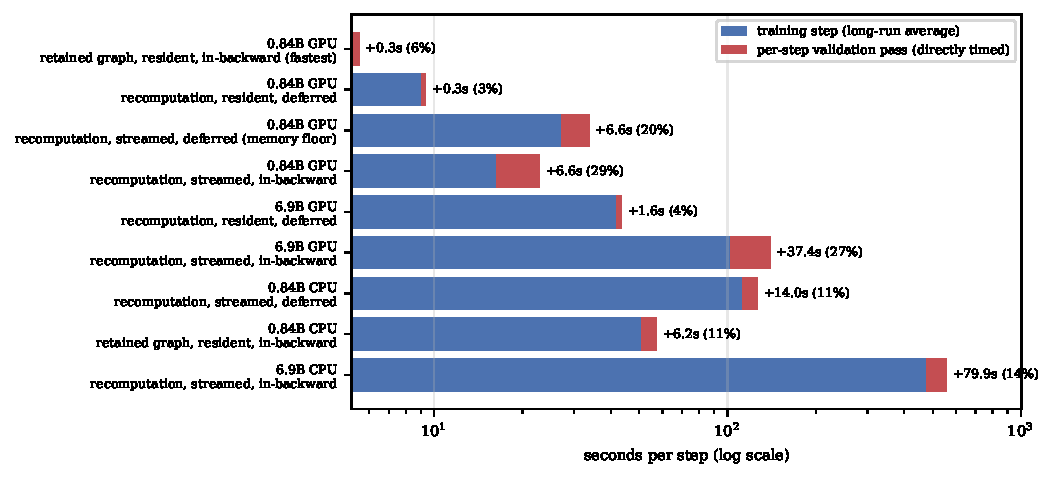
\includegraphics[width=\textwidth]{figures/fig_exp9_validation_cost.pdf}
\caption{The directly priced per-step validation pass (red) on top of the
training-only long-run step time (blue), per configuration. Adding the red
component converts a training-realistic step into the four-phase
measurement protocol's step.}
\label{fig:valcost}
\end{figure*}

% ============================================================================
\section{Exactness}\label{sec:exact}
% ============================================================================
Before any cost is reported, we establish that every mode computes the model
it claims to compute. All checks in this section run at the cost tier
(0.84B, $8{\times}2{\times}2{\times}8$) with the paper-true store bindings,
each mode under its own protocol: deferred modes with global gradient-norm
clipping at 1.0, optimizer-in-backward modes without (Sec.~\ref{sec:torchrt}).
All deltas are worst-case ($\max|\Delta|$ over all elements, and over all
modes in the row's scope), not averages.

\subsection{Training Identity}\label{sec:trainexact}
Table~\ref{tab:identity} summarizes the campaign. Forward hidden states
agree with the unsegmented reference to $1.2{\times}10^{-5}$ after 36 layers
of fp32 accumulation; per-slice gradients agree to $1.1{\times}10^{-8}$;
post-step parameters after one and after four full AdamW steps agree to the
$10^{-5}$ level across \emph{all} 840M parameters, reassembled and compared
element by element. With dropout on, where no reference with identical masks
exists, we verify determinism (repeat runs of the same mode) and cross-mode
agreement (streamed, recomputed, and resident execution draw identical masks
and produce gradients agreeing to $3.2{\times}10^{-9}$). On CPU the backward
is bit-deterministic, and the optimizer-in-backward modes are \emph{bit-identical}
to their deferred twins ($\Delta=0.0$); on GPU determinism is limited only by
atomic-accumulation ordering at ${\sim}2{\times}10^{-9}$.

\begin{table}[t]
\caption{Training identity at 0.84B. Worst-case $\max|\Delta|$ over all
modes in scope; ``vs.\ ref.''\ compares against the unsegmented full model
on identical seeds. The control rows run no segmentation code: the
full model against itself, batch of 2 versus twice-accumulated batch of 1,
in pure PyTorch.}
\label{tab:identity}
\centering
\begin{tabular}{@{}lcc@{}}
\toprule
Check (scope) & GPU & CPU \\
\midrule
Forward hidden state vs.\ ref.\ (all 12 modes) & $1.2{\times}10^{-5}$ & $3.8{\times}10^{-6}$ \\
Gradient slices vs.\ ref.\ (no-dropout, deferred) & $1.1{\times}10^{-8}$ & $3.5{\times}10^{-9}$ \\
Params.\ after 1 step vs.\ ref.\ (deferred, clip) & $5.4{\times}10^{-5}$ & $1.4{\times}10^{-5}$ \\
Params.\ after 4 steps vs.\ ref.\ (deferred, clip) & $5.4{\times}10^{-5}$ & $1.1{\times}10^{-4}$ \\
Params.\ after 4 steps vs.\ ref.\ (in-backward, no clip) & $3.8{\times}10^{-4}$ & $1.8{\times}10^{-4}$ \\
Backward determinism, repeat run (dropout on) & $2.3{\times}10^{-9}$ & $\mathbf{0.0}$ \\
Cross-mode gradients vs.\ anchor (dropout on) & $3.2{\times}10^{-9}$ & $1.8{\times}10^{-9}$ \\
In-backward vs.\ deferred twin, all params.\ (dropout on) & $1.4{\times}10^{-4}$ & $\mathbf{0.0}$ \\
\midrule
\emph{Control:} framework vs.\ itself, gradients (clip) & $2.2{\times}10^{-7}$ & $1.5{\times}10^{-8}$ \\
\emph{Control:} framework vs.\ itself, step (clip) & $3.5{\times}10^{-5}$ & $3.1{\times}10^{-6}$ \\
\emph{Control:} framework vs.\ itself, step (no clip) & $2.3{\times}10^{-4}$ & $3.1{\times}10^{-5}$ \\
\bottomrule
\end{tabular}
\end{table}

Two observations turn these numbers into a claim. First, the apparent gap
between gradient-level ($10^{-8}$) and step-level ($10^{-5}$) agreement is
fully explained: Adam divides each gradient by its running magnitude, so for
parameters whose gradient sits at the float noise floor, a $10^{-8}$
difference is amplified to a visible fraction of the learning rate. Every
element with step delta above $10^{-5}$ has $|g|<10^{-7}$; applying the
update rule to the two gradient sets reproduces the observed deltas with
residual below $10^{-9}$; and the worst delta, $5{\times}10^{-5}$, is far
below $2\cdot\text{lr}=6{\times}10^{-4}$, the scale at which an update could
be meaningfully wrong. Second, the \emph{control}: running the framework
against itself---the full model, batch of 2 versus twice-accumulated batch
of 1, zero segmentation code---produces \emph{larger} deviations than
segmentation does. The control's gradients differ by $2.2{\times}10^{-7}$
(ours: $1.1{\times}10^{-8}$) and its clipped step leaves 154 elements above
$10^{-5}$ (ours: 16). The $10^{-5}$-class step deltas are the fp32
execution-order floor of the framework itself, and segmented execution sits
at or below it. This is the empirical content of
Theorem~\ref{thm:invariance}. The control also isolates the effect of
clipping---the no-clip protocol is an order noisier in both worlds---which
is one more reason the deferred schedule with global clipping remains the
default recipe.

\subsection{Inference Identity}\label{sec:inferexact}
All four inference modes (streaming $\times$ KV cache), on both devices,
produce greedy decodes \emph{identical token for token} with the full-model
reference over a battery of fixed prompts, 20 tokens each (prefill deltas
$4.6{\times}10^{-6}$ GPU, $3.6{\times}10^{-6}$ CPU; no divergence at any
decode position). Recomputing the prefix without a cache and streaming
segments from the store change where tensors live, not what is computed.

\subsection{Matched-Pair Learning}\label{sec:quality}
The identity checks bound one step; the remaining question is whether
trajectories diverge over a full training run. At the accuracy tier, under
one protocol (10 epochs, batch 64, identical seeds), we train the full model
and two segmented modes end to end (Table~\ref{tab:quality},
Fig.~\ref{fig:curves}). Test token
accuracy agrees to three decimals, and the difference between full and
segmented ($4{\times}10^{-4}$) is the same size as the difference between
the two segmented modes ($3{\times}10^{-4}$)---a pair whose gradients are
\emph{proven} to agree at $10^{-8}$ in Table~\ref{tab:identity}. The
residual spread is seed-level noise, not a segmentation effect.

\begin{table}[t]
\caption{Matched-pair training at the accuracy tier: identical data, seeds,
and schedule; 11{,}654 test examples.}
\label{tab:quality}
\centering
\begin{tabular}{@{}lcc@{}}
\toprule
Configuration & Best val.\ loss & Test token acc. \\
\midrule
Full model (unsegmented) & --- & 0.9954 \\
Segmented, retained graph & 0.0191 & 0.9950 \\
Segmented, recomputation & 0.0190 & 0.9953 \\
\bottomrule
\end{tabular}
\end{table}

\begin{figure*}[t]
\centering
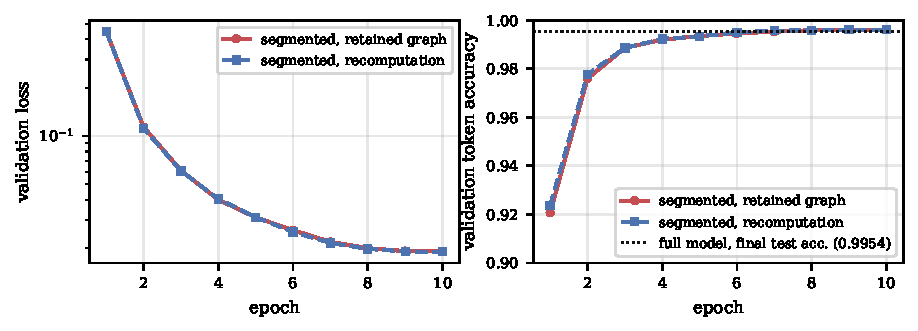
\includegraphics[width=\textwidth]{figures/learning_curves.pdf}
\caption{Matched-pair training at the accuracy tier (identical data, seeds,
schedule). Left: per-epoch validation loss of the two segmented modes---the
curves are indistinguishable, as the gradient-level identity of
Table~\ref{tab:identity} predicts. Right: validation token accuracy, with
the full model's final test accuracy as reference.}
\label{fig:curves}
\end{figure*}

\subsection{Prediction Agreement Across Engines}\label{sec:predagree}
Finally, the strictest end-to-end statement: from one segmented checkpoint,
nine serving pipelines---the segmented PyTorch engine in all four inference
modes, the exported unsegmented model, and the PyTorch-free ONNX runtime in
four placement configurations on both providers---produce \emph{identical
predictions on all 11{,}654 test examples} (exact-match 0.9548 in every
cell, agreement $11{,}654/11{,}654$, zero disagreements at the token level).
The independently trained full model, evaluated under the identical
protocol, reaches an exact-match of 0.9556---the two training paths land
within $0.1\%$ of each other at the prediction level as well.
Under equal-length batching there is no measurable accuracy cost to
segmentation, export, or engine substitution: the deployment stack is free
to choose its runtime by memory and latency alone.

% ============================================================================
\section{Evaluation}\label{sec:eval}
Exactness being settled, evaluation asks four questions. \textbf{Q1
(capability):} does temporal multiplexing move the wall---do models whose
full-model training aborts on the device train under segmentation?
\textbf{Q2 (budget):} how far down does device memory go, at what time
price, and is the trade a readable menu? \textbf{Q3 (serving):} what does
the same partition buy at inference, in both runtimes? \textbf{Q4
(structure):} how do the costs move with model size and partition
granularity, and where does the time go? Unless noted, training cells are
medians of three isolated runs at batch 4, sequence 512; inference cells use
a 256-token prompt and greedy decode, batch 1.

\subsection{Anchors and Baselines at 0.84B}\label{sec:anchors}
Table~\ref{tab:compare} sets the stage on one 40~GB A100. Full-model
training peaks at 25.4~GB; DeepSpeed ZeRO-Offload lowers this to 21.5~GB
(stage 2) and 23.6~GB (stage 3) at $2.9$--$4.1\times$ the step
time---consistent with its design point, which offloads optimizer state and
parameters but leaves the working activations and gradients of the
\emph{whole layer stack} on the device. The naive segmented anchor---the
partition with every dial off---lands at 18.2~GB: the partition alone
already bounds attention and feed-forward transients below both ZeRO
configurations, but the retained graph and resident weights still dominate.
The dials do the rest: the fastest streamed mode reaches 1.08~GB,
$23.5\times$ below full-model training and $19.9\times$ below the measured
ZeRO-Offload floor, and a finer partition reaches 890~MB
(Sec.~\ref{sec:gran}). On CPU the same story holds against the full model:
26.9~GB falls to 1.29~GB ($20.9\times$) at $4.7\times$ the step time.

\begin{table}[t]
\caption{Training at 0.84B on one A100-40GB (batch 4, seq.\ 512). Medians
of three isolated runs. ZeRO-Offload baselines measured on the same node
and model.}
\label{tab:compare}
\centering
\begin{tabular}{@{}lrr@{}}
\toprule
Configuration & Device peak & Step time \\
\midrule
Full model (retained graph) & 25.4\,GB & 0.72\,s \\
ZeRO-Offload stage 2 & 21.5\,GB & 2.1\,s \\
ZeRO-Offload stage 3 & 23.6\,GB & 2.9\,s \\
Naive segmented (partition only) & 18.2\,GB & 6.2\,s \\
Segmented, fastest ($\le$12\,GB class) & 11.5\,GB & 3.9\,s \\
Segmented, smallest (standard partition) & 1.08\,GB & 28.3\,s \\
Segmented, smallest (fine partition) & 0.89\,GB & 30.8\,s \\
\bottomrule
\end{tabular}
\end{table}

\subsection{The Mode Grid at 0.84B}\label{sec:grid}
Table~\ref{tab:grid} is the paper's centerpiece: all 12 training modes on
both devices, measured under the four-phase protocol (its times are
protocol-inclusive and comparable \emph{across} rows; deployment step
times are in Table~\ref{tab:sustainedtrain}); Fig.~\ref{fig:frontier} plots the same cells as a
memory--time frontier against the anchors, and Fig.~\ref{fig:traces} shows
the device-memory timeline of three representative modes. Reading the grid
as a menu:

\begin{figure*}[t]
\centering
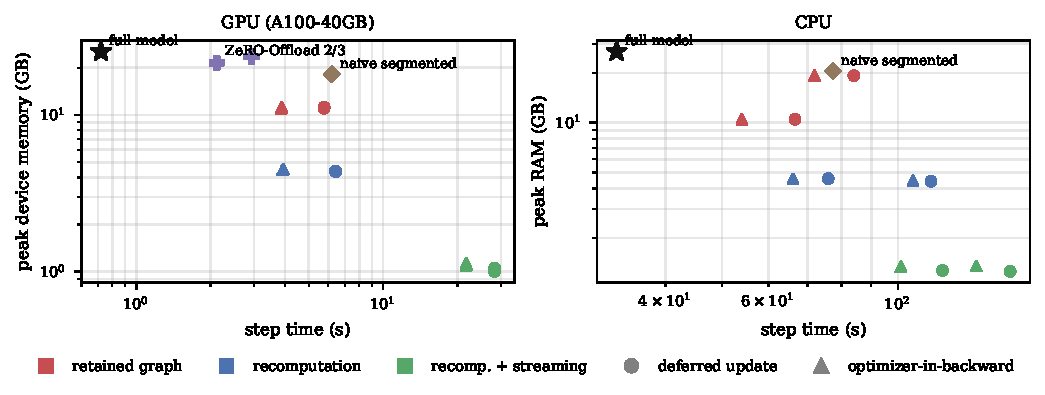
\includegraphics[width=\textwidth]{figures/frontier_train.pdf}
\caption{The training memory--time frontier at 0.84B (log--log; every point
computes the same model). Left: GPU, with the full-model, naive-segmented,
and measured ZeRO-Offload anchors. Right: CPU. Color encodes the memory
regime (retained graph / recomputation / recomputation + streaming); marker
shape encodes the update schedule.}
\label{fig:frontier}
\end{figure*}

\begin{figure}[t]
\centering
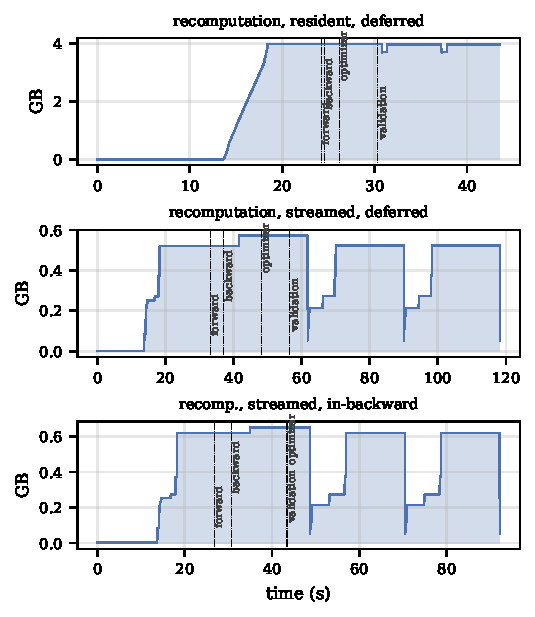
\includegraphics[width=\columnwidth]{figures/traces_gpu.pdf}
\caption{Reserved device memory over one measured run (build, warmup, three
steps, validation) for three modes at 0.84B. The plateaus and phase
boundaries make the residency invariant visible: streaming caps the curve
at the segment scale, and the in-backward schedule removes the optimizer
phase entirely.}
\label{fig:traces}
\end{figure}

\begin{table*}[t]
\caption{The 12 training modes at 0.84B (medians of three isolated runs;
batch 4, seq.\ 512). Graph: retained vs.\ recomputed; weights: resident
vs.\ streamed; update: deferred sweep vs.\ optimizer-in-backward. GPU
columns: peak device memory, host-side store (RSS), step time, optimizer
phase. CPU columns: peak RAM, step time, optimizer phase. Every row
computes the same model (Sec.~\ref{sec:exact}).}
\label{tab:grid}
\centering
\small
\begin{tabular}{@{}cccc rrrr rrr@{}}
\toprule
 & & & & \multicolumn{4}{c}{GPU (A100-40GB)} & \multicolumn{3}{c}{CPU} \\
\cmidrule(lr){5-8}\cmidrule(l){9-11}
Dropout & Graph & Weights & Update & VRAM & Host & Step & Opt.\ & RAM & Step & Opt.\ \\
 & & & & (MB) & (GB) & (s) & (s) & (MB) & (s) & (s) \\
\midrule
\checkmark & retained & resident & deferred & 11{,}486 & 19.8 & 5.77 & 4.13 & 19{,}692 & 84.0 & 27.9 \\
\checkmark & recomp. & resident & deferred & 4{,}488 & 20.9 & 6.41 & 4.07 & 4{,}520 & 113.9 & 27.1 \\
\checkmark & recomp. & streamed & deferred & 1{,}080 & 19.8 & 28.27 & 8.24 & 1{,}288 & 155.6 & 35.8 \\
--- & retained & resident & deferred & 11{,}316 & 20.7 & 5.76 & 4.10 & 10{,}736 & 66.6 & 29.7 \\
--- & recomp. & resident & deferred & 4{,}464 & 21.2 & 6.43 & 4.17 & 4{,}694 & 76.0 & 28.0 \\
--- & recomp. & streamed & deferred & 1{,}030 & 19.6 & 28.26 & 8.29 & 1{,}304 & 119.2 & 40.5 \\
\checkmark & retained & resident & in-backward & 11{,}454 & 19.0 & 3.89 & 0.11 & 19{,}702 & 72.0 & 0.03 \\
\checkmark & recomp. & resident & in-backward & 4{,}608 & 17.6 & 3.94 & 0.10 & 4{,}569 & 106.1 & 0.03 \\
\checkmark & recomp. & streamed & in-backward & 1{,}158 & 15.8 & 21.69 & 0.11 & 1{,}388 & 136.2 & 0.03 \\
--- & retained & resident & in-backward & 11{,}284 & 18.0 & 3.87 & 0.11 & 10{,}747 & 54.1 & 0.03 \\
--- & recomp. & resident & in-backward & 4{,}584 & 17.8 & 3.92 & 0.11 & 4{,}669 & 66.1 & 0.03 \\
--- & recomp. & streamed & in-backward & 1{,}126 & 16.3 & 21.69 & 0.11 & 1{,}374 & 101.1 & 0.03 \\
\bottomrule
\end{tabular}
\end{table*}

\textbf{Three memory plateaus.} The graph and weight dials set three clean
GPU plateaus---${\sim}11.4$~GB (retained graph), ${\sim}4.5$~GB
(recomputation), ${\sim}1.1$~GB (recomputation + streaming)---each
$2.2$--$4.1\times$ below the last, and the update schedule barely moves
memory. The same plateaus appear on CPU RAM.

\textbf{Optimizer-in-backward removes a phase, not a percentage.} The
deferred optimizer sweep costs 4.1~s per step on GPU and 28~s on CPU; the
in-backward schedule collapses it to 0.1~s and 0.03~s respectively---it is
not faster bookkeeping but the deletion of one full traversal of 840M
parameters through the store. It makes the fastest mode 3.9~s
($5.4\times$ full-model time at less than half its memory) and cuts the
smallest-memory streamed mode from 28.3~s to 21.7~s ($30\times$) at
1.16~GB.

\textbf{Dropout's memory price is regime-dependent.} On GPU, dropout adds
only ${\sim}0.2$~GB in every regime (fused kernels keep masks small; the
full model pays 1.26~GB for the same setting). On CPU with a retained
graph, dropout \emph{doubles} peak RAM (19.7 vs.\ 10.7~GB): eager CPU
autograd materializes full-width mask and product tensors in the graph.
Under recomputation the penalty collapses to ${\sim}0.2$~GB on both
devices---recomputation pays for dropout's memory, then RNG replay
(Sec.~\ref{sec:torchrt}) pays back its correctness.

\textbf{The store is part of the bargain.} A 1.1~GB streamed GPU run
carries a 16--20~GB host-side store (parameters, gradients, moments,
records); the CPU rows carry the same state on disk. Nothing is free; the
claim is that the \emph{constrained} resource is spent at 4--30$\times$
less while total system memory is repartitioned, not inflated.

\subsection{Inference at 0.84B}\label{sec:infereval}
Table~\ref{tab:infer} reports both runtimes, and Fig.~\ref{fig:inferfrontier}
plots them as a serving frontier.

\begin{figure*}[t]
\centering
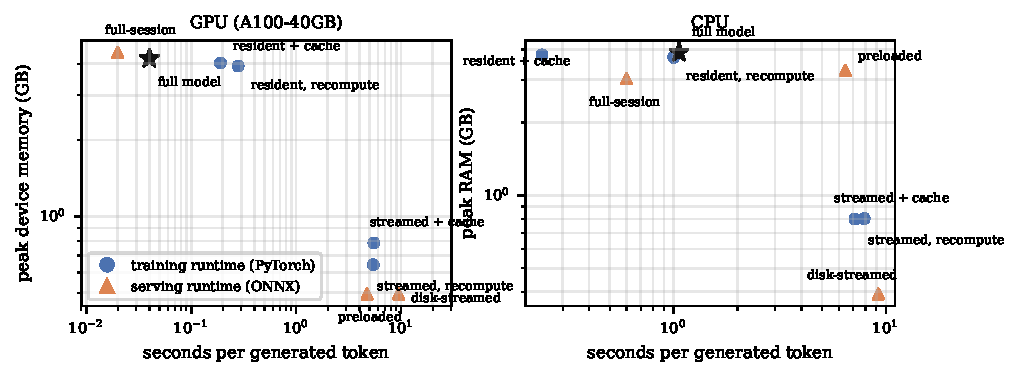
\includegraphics[width=\textwidth]{figures/inference_frontier.pdf}
\caption{The serving frontier at 0.84B (log--log): memory against decode
latency for both runtimes and the full-model anchor, on GPU (left, device
memory) and CPU (right, RAM). All points produce identical predictions
(Sec.~\ref{sec:predagree}).}
\label{fig:inferfrontier}
\end{figure*} In the training runtime, the
full-model reference decodes at 0.038~s/token in ${\sim}4$~GB; resident
segmented execution matches its memory (weights dominate both) and pays
$5.1\times$ in per-segment launch overhead at this small scale---a price
that inverts at 7B (Sec.~\ref{sec:scale}), and that on CPU is already
inverted at 0.84B: with the KV cache, resident segmented decoding is
$4.4\times$ \emph{faster} than the no-cache full reference (0.238 vs.\
1.056~s/token). Streaming with KV cache drops
device memory to 804~MB, and dropping the cache too reaches 660~MB at
5.4~s/token. The PyTorch-free runtime spans the same trade with less
overhead at both ends: the full-session export is the fastest cell in the
paper (0.018~s/token on GPU), and the disk-streamed weights-as-inputs mode
serves in \textbf{401~MB total} on CPU---no GPU, no PyTorch, no
host-resident weight copy---at 9.2~s/token. The excluded baked-per-segment
design (11.6~GB, Sec.~\ref{sec:onnxrt}) is dominated at both ends.

Sustained serving (Table~\ref{tab:sustainedserve},
Fig.~\ref{fig:sustainedserve}) extends each mode to 500--2{,}000
consecutive requests: the resident 6.9B server holds exactly 27.8~GB
(reserved) for 1{,}000 requests, and the PyTorch-free disk-streamed server
answers 500 requests inside 377--389~MB---12~MB of runtime-arena wobble, no
trend, no session leak. Under this instrumentation-free protocol the cache
modes' latency is \textbf{0.031~s/token} (0.84B) and \textbf{0.035~s/token}
(6.9B): the per-operation tracer inside the mode-comparison protocol
inflates sub-second decoding $5.9\times$ (measured back-to-back on one
node, Sec.~\ref{sec:longhorizon}) while slow modes agree within
2--16\%. Table~\ref{tab:infer} therefore remains the \emph{relative}
comparison across modes under equal instrumentation; deployment latencies
are those of Table~\ref{tab:sustainedserve}.

\begin{table}[t]
\caption{Long-horizon serving: sustained footprint (GPU: reserved + CUDA
context; CPU: resident set), band over the whole session, and
instrumentation-free latency.}
\label{tab:sustainedserve}
\centering
\scriptsize
\setlength{\tabcolsep}{3pt}
\begin{tabular}{@{}lrrrr@{}}
\toprule
Serving mode & Requests & Footprint & Band & s/token \\
\midrule
0.84B GPU resident + KV cache & 2{,}000 & 4{,}298\,MB & 0\,MB & 0.031 \\
0.84B GPU streamed + recompute & 500 & 656\,MB & 0\,MB & 5.00 \\
0.84B CPU ONNX, disk-streamed & 500 & 377--389\,MB & 12\,MB & 9.06 \\
6.9B GPU resident + KV cache & 1{,}000 & 28{,}336\,MB & 0\,MB & 0.035 \\
\bottomrule
\end{tabular}
\end{table}

\begin{figure*}[t]
\centering
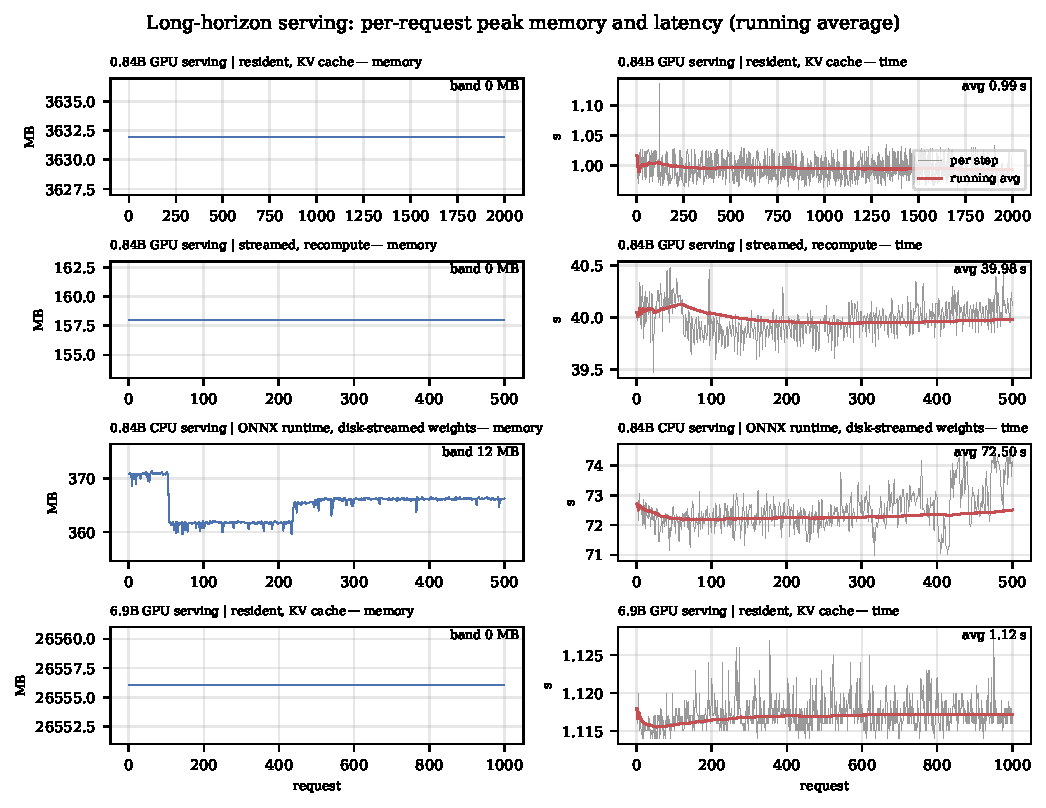
\includegraphics[width=\textwidth]{figures/fig_exp8_serving.pdf}
\caption{Long-horizon serving, per experiment: per-request peak memory and
latency with its running average, over the full session.}
\label{fig:sustainedserve}
\end{figure*}

\begin{table}[t]
\caption{Inference at 0.84B (prompt 256, greedy decode, batch 1; medians
of three). GPU cells: device peak / host RSS / s per token; CPU cells:
RAM / s per token. All rows share the per-operation tracing
instrumentation; deployment latencies for the fast modes are in
Table~\ref{tab:sustainedserve}.}
\label{tab:infer}
\centering
\small
\begin{tabular}{@{}lrrr rr@{}}
\toprule
 & \multicolumn{3}{c}{GPU} & \multicolumn{2}{c}{CPU} \\
\cmidrule(lr){2-4}\cmidrule(l){5-6}
Mode & MB & Host & s/tok & MB & s/tok \\
\midrule
\multicolumn{6}{@{}l}{\emph{Training runtime (PyTorch)}} \\
Full model (no cache) & 4{,}292 & 3.7\,GB & 0.038 & 3{,}981 & 1.056 \\
Resident + KV cache & 4{,}122 & 4.2\,GB & 0.192 & 3{,}891 & 0.238 \\
Resident, recompute & 4{,}008 & 4.2\,GB & 0.283 & 3{,}800 & 0.996 \\
Streamed + KV cache & 804 & 4.3\,GB & 5.50 & 819 & 7.14 \\
Streamed, recompute & 660 & 4.3\,GB & 5.43 & 822 & 7.90 \\
\multicolumn{6}{@{}l}{\emph{Serving runtime (ONNX, PyTorch-free)}} \\
Full-session & 4{,}534 & 0.7\,GB & 0.018 & 3{,}100 & 0.603 \\
Preloaded & 506 & 3.8\,GB & 4.75 & 3{,}346 & 6.43 \\
Disk-streamed & 506 & 0.8\,GB & 9.47 & \textbf{401} & 9.20 \\
\bottomrule
\end{tabular}
\end{table}

\subsection{Scale: Moving the Wall}\label{sec:scale}
Table~\ref{tab:scale} answers Q1, on both device
classes: a CPU-only node trains the 6.9B model in 9.3~GB of RAM (where
full-model training needs 111.6~GB), and the 40~GB accelerator carries
every size that aborts larger devices.

 On the 40~GB device, full-model training
fits only up to 1.5B (39.0~GB---already at the edge); at 3B it aborts, and
an H100 measurement shows why: 67.6~GB. At 5B it aborts on an 80~GB device,
and at 6.9B \emph{even the 94~GB H100 aborts}. Segmented execution trains
all of them on the single 40~GB card, three ways. Resident with
recomputation, 6.9B trains at 28.5~GB and 58.1~s per step---a model whose
conventional training exceeds the largest single accelerator sold, on a
mid-range card, with $71\%$ of the device left over at 3B (14.0~GB).
Sustained training confirms every cell is representative rather than a
snapshot (Table~\ref{tab:sustainedtrain}, Fig.~\ref{fig:sustainedtrain}):
each headline mode runs 128--2{,}048 consecutive steps over 3--17 hours
under the training-realistic protocol of Sec.~\ref{sec:longhorizon}. On
GPU the per-step peak is \emph{identical to the byte} on every step of
every run---including 1{,}024 steps of the 6.9B resident configuration at
29.2~GB and 2{,}048 steps of the memory-floor mode---with no allocator
trimming. On CPU the resident set oscillates between allocator plateaus
within a bounded band ($\le$691~MB at 0.84B; transient first-touch
excursions at 6.9B settle within ten steps) with no trend. Step times are
stationary; their residual variance is co-tenant noise on the shared nodes
(Sec.~\ref{sec:longhorizon}), reported as the p5--p95 spread.

\begin{table}[t]
\caption{Long-horizon training: sustained peak and band in MB (GPU:
reserved + CUDA context; CPU: resident set), the training-only long-run
step time, and the directly priced per-step validation pass (+val.) that
converts to the four-phase protocol.}
\label{tab:sustainedtrain}
\centering
\scriptsize
\setlength{\tabcolsep}{2.5pt}
\begin{tabular}{@{}lrrrrr@{}}
\toprule
Mode & Steps & Peak & Band & Step & +val. \\
\midrule
\multicolumn{6}{@{}l}{\emph{0.84B, GPU}} \\
\enspace retained, resident, in-backward & 2{,}048 & 11{,}968 & 0 & 5.23\,s & +0.3\,s \\
\enspace recompute, resident, deferred & 2{,}048 & 4{,}663 & 0 & 9.05\,s & +0.3\,s \\
\enspace recompute, streamed, deferred & 2{,}048 & 1{,}142 & 0 & 27.11\,s & +6.6\,s \\
\enspace recompute, streamed, in-backward & 2{,}048 & 1{,}172 & 0 & 16.28\,s & +6.6\,s \\
\multicolumn{6}{@{}l}{\emph{6.9B, GPU}} \\
\enspace recompute, resident, deferred & 1{,}024 & 29{,}687 & 0 & 41.90\,s & +1.6\,s \\
\enspace recompute, streamed, in-backward & 512 & 2{,}799 & 0 & 102.2\,s & +37.4\,s \\
\multicolumn{6}{@{}l}{\emph{0.84B, CPU}} \\
\enspace recompute, streamed, deferred & 512 & 2{,}087 & 349 & 112.5\,s & +14.0\,s \\
\enspace retained, resident, in-backward & 1{,}024 & 21{,}134 & 691 & 50.95\,s & +6.2\,s \\
\multicolumn{6}{@{}l}{\emph{6.9B, CPU}} \\
\enspace recompute, streamed, in-backward & 128 & 7{,}932 & 1{,}251 & 478.0\,s & +79.9\,s \\
\bottomrule
\end{tabular}
\end{table}

\begin{figure*}[p]
\centering
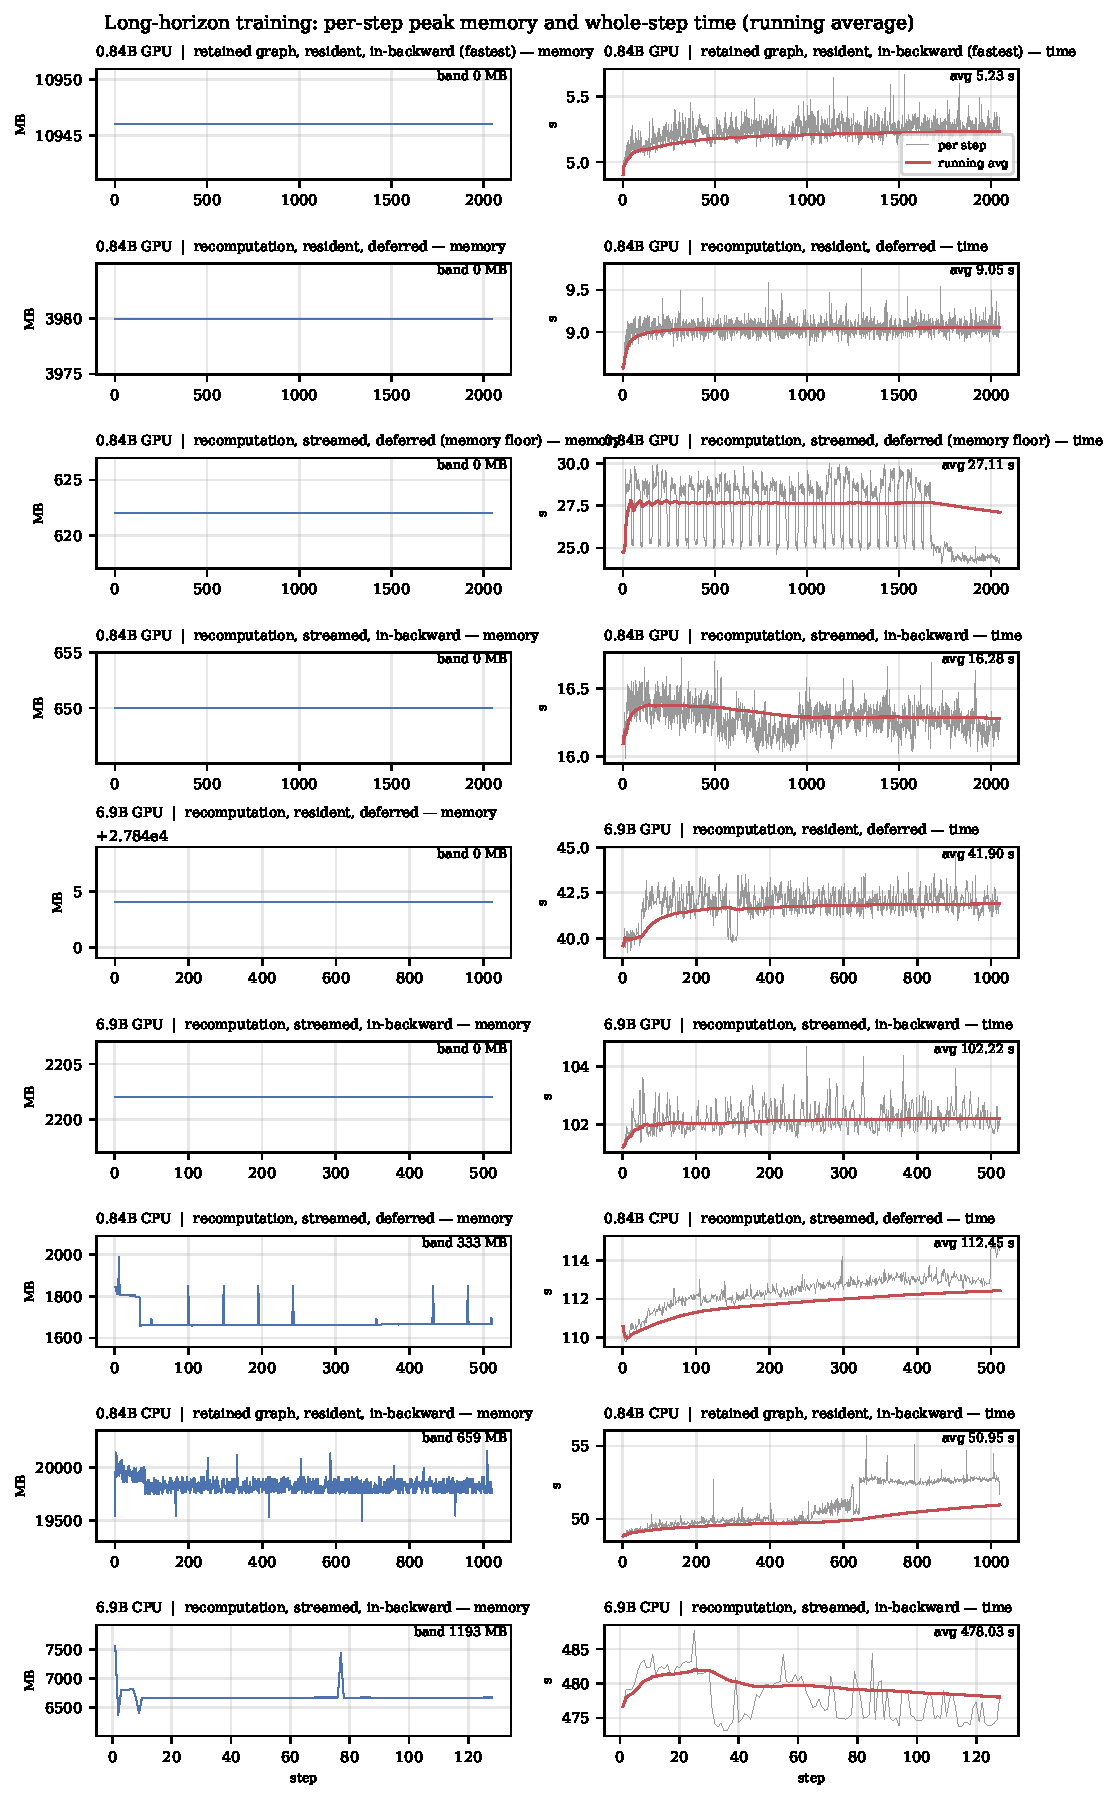
\includegraphics[height=0.94\textheight]{figures/fig_exp8_training.pdf}
\caption{Long-horizon training, per experiment: per-step peak memory
(left; band annotated) and whole-step wall time with its running average
(right), from the first to the last step.}
\label{fig:sustainedtrain}
\end{figure*}
Streamed, the same models train in 1.7--2.6~GB (deferred) or at
$1.3\times$ less time with in-backward updates; device memory grows only
through the widest segment---from 0.84B to 6.9B ($8.2\times$ the
parameters), streamed VRAM grows just $2.4\times$. The host store grows in
proportion to the model (up to ${\sim}107$~GB at 6.9B), which is the
explicit bargain: capacity is bought from the abundant tier. On CPU, 6.9B
full-model training needs 111.6~GB of RAM; streamed in-backward training
needs 9.3~GB ($12\times$ less) at $4.0\times$ the time.

\begin{table}[t]
\caption{Training at scale on one A100-40GB (top) and one CPU node
(bottom). ``Full'' is unsegmented training; OOM = allocation failure, with
the H100-94GB result in parentheses. Streamed cells: deferred /
in-backward step times.}
\label{tab:scale}
\centering
\scriptsize
\setlength{\tabcolsep}{3pt}
\begin{tabular}{@{}lrrrr@{}}
\toprule
Model & Full & Resident seg. & \multicolumn{2}{c}{Streamed seg.} \\
 & & & VRAM & Step (s) \\
\midrule
1.5B & 39.0\,GB / 1.3\,s & 17.4\,GB / 10.3\,s & 1.3\,GB & 64.7 / 49.0 \\
3.1B & OOM (67.6\,GB) & 14.0\,GB / 26.6\,s & 1.7\,GB & 111.6 / 84.9 \\
5.1B & OOM ($>$80\,GB) & --- & 2.2\,GB & 184.5 / 137.0 \\
6.9B & OOM ($>$94\,GB) & 28.5\,GB / 58.1\,s & 2.6\,GB & 229.4 / 172.8 \\
\midrule
3.1B (CPU) & 59.3\,GB / 68\,s & --- & 2.9--3.5\,GB & 351 / 300 \\
6.9B (CPU) & 111.6\,GB / 159\,s & --- & 9.3--10.8\,GB & 735 / 629 \\
\bottomrule
\end{tabular}
\end{table}

At inference the wall moves the same way, and the latency picture inverts
in segmentation's favor: resident segmented decoding with KV cache is
essentially \emph{size-independent} on GPU---0.21, 0.21, 0.19~s/token at
1.5B, 3.1B, and 6.9B---while the no-cache full-model reference grows from
0.39 to 1.57~s/token. The smallest streamed mode serves 6.9B in 1.6~GB of
device memory (33~s/token), and on CPU in 2.4~GB.

\subsection{Granularity}\label{sec:gran}
The partition is a dial of its own. At 0.84B, coarsening to
$2{\times}1{\times}1{\times}2$ or refining to $16{\times}4{\times}4{\times}16$
changes segment count by $64\times$ end to end, yet: the recomputation
plateau barely moves (5.2, 4.5, 4.5~GB); the streamed floor tracks the
widest segment---2.14~GB coarse, 1.08~GB standard, \textbf{890~MB} fine at
30.8~s---exactly as Eq.~(\ref{eq:memlaw}) predicts; and the fastest
resident mode degrades gracefully with segment count (5.8, 3.9, 10.5~s),
locating the sweet spot at moderate granularity. Inference mirrors it:
coarse partitions decode fastest (0.12~s/token), fine partitions serve
smallest (598~MB streamed).

\subsection{From Temporal to Spatial: An Analytic Bridge}\label{sec:spatial}
Nothing in the partition is specific to time-multiplexing: the same cuts
are the cuts of tensor parallelism, and the measured quantities translate
(Table~\ref{tab:spatial}). A spatial deployment of the standard 0.84B
partition over $P$ devices holds one segment per device where we hold one
per \emph{time slot}: its per-device memory is our measured segment
residency plus reassembly activations; our sequential step time is an upper
bound that parallel execution divides by up to $P$, minus collective costs
that replace our store traffic. The temporal measurements therefore give a
device-count-free lower envelope for the spatial family---one this paper
validates on a single device, with the multi-device instantiation left as
engineering.

\begin{table}[t]
\caption{The temporal--spatial correspondence for one partition.}
\label{tab:spatial}
\centering
\small
\begin{tabular}{@{}lll@{}}
\toprule
Quantity & Temporal (this paper) & Spatial (tensor parallel) \\
\midrule
Parts co-resident & 1 (streamed floor) & $P$, one per device \\
Peak per device & Eq.~(\ref{eq:memlaw}), measured & same law per rank \\
Step time & $\sum_i t_i$, measured & $\max_i t_i$ + collectives \\
Join operations & local concat/add & all-gather / all-reduce \\
Transport & host/disk store & interconnect \\
\bottomrule
\end{tabular}
\end{table}
% ============================================================================
\section{Cost Model}\label{sec:model}
% ============================================================================
The structure observed in Sec.~\ref{sec:eval} compresses into two
first-order laws for the streamed deferred mode on the pinned A100 node.
With $P$ the parameter count in billions, $N$ the total number of segments
($N = L(A{+}M{+}1) + E + H$), and $s_v$ the vocabulary-tied slice pair of
Eq.~(\ref{eq:memlaw}):
\begin{align}
T &= 2.04 + 33.97\,P + 0.0094\,N \quad[\text{s/step}],\label{eq:timelaw}\\
M &= 533 + 5.26\,s_v + 0.179\,d_\text{model} \quad[\text{MB}].\nonumber
\end{align}
The coefficients are physical. Time: 34~s per billion parameters is the
marginal cost of sweeping every parameter through the device three times
per step (forward, backward, update)---transport plus small-kernel compute
plus synchronous orchestration, a split Sec.~\ref{sec:disc} quantifies;
9.4~ms per segment is the fixed transaction cost of one store fetch plus
kernel launches; the 2~s constant absorbs framework overhead. Memory: the slope on
$s_v$ bundles the resident slice with its gradient, transients, and
allocator rounding; the $d_\text{model}$ term carries shared parameters and
per-layer records. Both laws were fitted \emph{once} on the seven
configurations of Table~\ref{tab:costmodel} and then frozen. Both laws
describe the four-phase measurement protocol of Sec.~\ref{sec:discipline};
the long-horizon runs of Table~\ref{tab:sustainedtrain} give the
corresponding training-only step times, and the directly priced validation
pass (Fig.~\ref{fig:valcost}) converts between the two.

\begin{table}[t]
\caption{Cost-model accuracy. Fitted on the seven configurations above the
rule; the row below the rule is the held-out cell whose prediction was
committed to the repository before the job ran. Streamed deferred mode,
A100-40GB, medians of three.}
\label{tab:costmodel}
\centering
\small
\begin{tabular}{@{}lrrrr@{}}
\toprule
Configuration & \multicolumn{2}{c}{Memory (MB)} & \multicolumn{2}{c}{Step time (s)} \\
 & meas. & pred. & meas. & pred. \\
\midrule
0.84B, $8{\times}2{\times}2{\times}8$ & 1{,}080 & 1{,}101 & 28.3 & 32.3 \\
0.84B, $2{\times}1{\times}1{\times}2$ & 2{,}142 & 2{,}115 & 27.5 & 31.5 \\
0.84B, $16{\times}4{\times}4{\times}16$ & 890 & 932 & 30.8 & 33.8 \\
1.5B, $8{\times}2{\times}2{\times}8$ & 1{,}270 & 1{,}328 & 64.7 & 57.1 \\
3.1B, $8{\times}2{\times}2{\times}8$ & 1{,}748 & 1{,}668 & 111.6 & 108.8 \\
5.1B, $8{\times}2{\times}2{\times}8$ & 2{,}200 & 2{,}008 & 184.5 & 177.7 \\
6.9B, $8{\times}2{\times}2{\times}8$ & 2{,}550 & 2{,}349 & 229.4 & 236.5 \\
\midrule
3.1B, $16{\times}4{\times}4{\times}16$ (held out) & 1{,}268 & 1{,}330 & 102.7 & 110.3 \\
\bottomrule
\end{tabular}
\end{table}

\textbf{Accuracy, stated plainly.} In sample, the memory law is within
8.7\% everywhere; the time law is within 3.7\% at 3B and above, degrading
to $-12$\% at 1.5B and $+14$\% at 0.84B, where per-step costs that the law
does not model (validation passes, framework fixed costs) are no longer
negligible against the parameter term. We report these residuals rather
than adding terms: a two-coefficient time law that a practitioner can
evaluate on a napkin, accurate where the memory pressure actually is, is
the useful artifact.

\textbf{Sensitivity to batch and sequence length.} The memory law carries
no batch or sequence term, and a dedicated sweep shows why it can afford
not to (Table~\ref{tab:sensitivity}): across a $32\times$ token sweep at
0.84B---batch $\{1,4,8\}$ $\times$ sequence $\{128,256,512\}$, streamed
deferred mode, three isolated runs per cell---the floor moves only from
804~MB to 1{,}416~MB. The paper-protocol cell (batch 4, seq.\ 512)
reproduces the mode grid's 1{,}080~MB exactly from an independent run.
Activation transients contribute roughly 0.15~MB per token at the top of
the sweep; below ${\sim}2$k tokens per step the vocabulary-tied term
dominates and Eq.~(\ref{eq:memlaw}) applies unchanged, while larger token
budgets add the measured slope. Step \emph{time} is flatter still: within
the sweep's node, the $32\times$ token range moves the step by less than
$6\%$ (40.3--42.7~s under the four-phase protocol; the sweep's node ran
the paper-protocol cell at 41.5~s where the grid's node measured 28.3~s,
the node-placement spread of Sec.~\ref{sec:longhorizon})---the streamed
step is weight-traffic-bound, not token-bound, so the per-token cost of the smallest modes falls almost
linearly with batch size: batch 8 processes $8\times$ the tokens of batch
1 for $3\%$ more wall-clock.

\begin{table}[t]
\caption{Peak device memory (MB) of the streamed deferred mode at 0.84B
under a batch $\times$ sequence sweep (medians of three isolated runs).
Step time varies by less than 6\% across all nine cells.}
\label{tab:sensitivity}
\centering
\begin{tabular}{@{}lrrr@{}}
\toprule
 & seq.\ 128 & seq.\ 256 & seq.\ 512 \\
\midrule
batch 1 & 804 & 796 & 836 \\
batch 4 & 834 & 962 & 1{,}080 \\
batch 8 & 962 & 1{,}046 & 1{,}416 \\
\bottomrule
\end{tabular}
\end{table}

\textbf{Pre-registered validation.} The laws were then tested on a cell
that entered no fit: 3.09B parameters at the $16{\times}4{\times}4{\times}16$
partition---a size and granularity \emph{combination} never measured. The
prediction (110.3~s, 1{,}330~MB) was committed to the repository before the
job was submitted. Three isolated runs measured 102.4--103.0~s and
1{,}268~MB: the law over-predicted time by 7.1\% and memory by 4.9\%, both
conservative (the model errs toward over-provisioning). We consider this
the right epistemic standard for cost models: coefficients frozen in
public, then confronted with an unseen configuration.

% ============================================================================
\section{Discussion}\label{sec:disc}
% ============================================================================
\textbf{Where the time actually goes.} A bytes-moved account bounds what
streaming \emph{must} cost. At 0.84B the streamed deferred step transports
roughly 34~GB through the store interface: the 3.35~GB of fp32 weights
fetched twice (forward, backward), gradients parked and re-fetched, and the
optimizer sweep pulling and writing back weights and both Adam moments,
plus ${\sim}0.8$~GB of layer-input records. At a practical
${\sim}20$~GB/s over PCIe this is under 2~s---yet the measured step is
28.3~s. Transport is under $10\%$ of the step; the remaining $90\%$ is
synchronous orchestration: unoverlapped copies, per-segment Python
dispatch, small-kernel inefficiency, allocator churn. Two measured facts
corroborate the account. First, the in-backward schedule removes gradient
parking and the optimizer sweep's re-fetch---about $30\%$ of the traffic
\emph{and} one full pass of orchestration---and the step drops by $23\%$
(28.3${\to}$21.7~s). Second, the per-segment coefficient of
Eq.~(\ref{eq:timelaw}), 9.4~ms, is orders of magnitude above a
sub-millisecond DMA of a 32~MB slice. The conclusion cuts both ways: the
measured slowdowns are honest prices for a strict, verifiable residency
invariant executed synchronously---and most of the price is engineering
headroom, not algorithm. Prefetching the next segment during the current
one's compute would relax the residency floor from one segment to two and
attack the dominant term directly; we deliberately did not, because the
one-segment floor is the claim under test.

\textbf{What the time prices buy today.} The measured menu, taken at
face value on today's framework, already supports real work: the fastest
resident modes are everyday-practical (at 0.84B, a 10{,}000-step run is
${\sim}14$ hours); the streamed 6.9B modes support one- to two-day
fine-tunes of a thousand-odd steps in under 3~GB of device memory; and
batch amortization makes the streamed per-token cost nearly flat (batch~8
processes $8\times$ the tokens for $3\%$ more wall-clock,
Sec.~\ref{sec:model}). The 6.9B-on-CPU cell is a \emph{capability
boundary}, and we state its arithmetic plainly: at 478~s per step, an
overnight run is on the order of a hundred steps---suited to bounded
adaptation on private data, not to long training campaigns. Crucially,
these wall-clock prices are a property of the framework, not of the
method: the decomposition above attributes ${\sim}90\%$ of the streamed
step to synchronous orchestration by an engine built for the
memory-abundant regime, with transport itself bounded near 2~s. The memory
column of every table is what segmentation guarantees; the time column is
what today's PyTorch charges to honor it, and it shrinks with runtime
engineering, not with new mathematics.

\textbf{Segmentation equalizes hardware tiers.} Full-model training at
0.84B is $46\times$ slower on our CPU node than on the A100
(33.0 vs.\ 0.72~s). In the smallest streamed modes the ratio collapses to
$5$--$6\times$ (155.6 vs.\ 28.3~s deferred; 136.2 vs.\ 21.7~s
in-backward): once both devices spend most of the step on store traffic
and orchestration rather than dense math, the accelerator's FLOP advantage
is mostly idle. The effect is starkest in the serving runtime, where the
CPU \emph{beat} the A100 end to end on the full 11{,}654-example
evaluation at the accuracy tier (per-call weight upload dominates a small
model on the GPU provider). For the private-data settings of
Sec.~\ref{sec:intro}, this is the operative point: the hardware one
already owns is a viable training and serving substrate, and the penalty
for not owning an accelerator shrinks exactly in the regime this paper
targets.

\textbf{Engine independence as evidence of design.} The PyTorch-free
runtime is not a deployment convenience only; it is a falsifiable test of
the claim that segmented execution is a property of the \emph{computation}
rather than of a framework's autograd and allocator. The partition,
residency invariant, and reassembly algebra survived transplantation onto
a session-owned runtime with zero prediction divergence
(Sec.~\ref{sec:predagree}), and the one design that fought the
invariant---baked per-segment sessions---failed for a structural reason
(sessions own their weights) that the weights-as-inputs interface
resolves. We expect the same pattern, residency control through the graph
interface, to carry to other inference runtimes with session-owned
initializers.

\textbf{Security posture, stated precisely.} The security benefit of
segmented execution is \emph{data locality}: training and serving complete
on the device that owns the data, so the threats that motivate federated
and on-device learning---interception in transit, exposure to a serving or
training provider, gradient leakage to an aggregator---are removed by
construction rather than mitigated. We claim no more than that. An
adversary with physical or privileged access to the device itself (memory
inspection, side channels, model extraction from the local store) is
outside this paper's scope and must be addressed by the platform's own
protections; and once the federated extension of Sec.~\ref{sec:limits}
exchanges updates across devices, the standard defenses of that setting
(secure aggregation, differential privacy) become necessary again. The
mechanism's contribution to security is therefore precise and bounded: it
makes local execution \emph{possible} on hardware that could not
previously train, eliminating the need to export data in the first place.

\textbf{The dials become the runtime's job.} Sec.~\ref{sec:exact} makes
every mode safe and Sec.~\ref{sec:model} makes every mode predictable;
together they turn mode selection into scheduling. A runtime given a
device budget and a deadline can invert the two laws: choose the coarsest
partition whose $M$ fits the budget, then the fastest update schedule the
recipe tolerates (in-backward where global clipping is dispensable), and
switch modes between phases---resident for pre-training bursts on rented
hardware, streamed in-backward for on-device fine-tuning, disk-streamed
serving after export. Nothing in the lattice is a hyperparameter: no
choice affects what is learned, only where bytes sit and how long steps
take. Memory, in other words, is scheduled like CPU time---which is the
thesis of the paper restated as a systems roadmap.

% ============================================================================
\section{Limitations and Future Work}\label{sec:limits}
% ============================================================================
\textbf{Scope of the numbers.} All measurements are fp32. Mixed precision
and quantized optimizer states are orthogonal to the partition and would
shrink absolute footprints on \emph{both} sides of every comparison,
shifting the out-of-memory boundaries of Table~\ref{tab:scale} without
changing the structure of the memory law. Wall-clock results are specific
to the measured PCIe- and NVMe-class node and, on the shared partition,
carry co-tenant variance, which we quantify rather than control; the cost
model's segment and parameter coefficients would refit on other hardware,
its form should not.
Inference is batch-one greedy decoding with a single-sequence KV path;
batched serving under the residency invariant is unexplored. The exactness
matrix is exhaustive at the mode level but the architecture is one family:
a GPT decoder. The four cut planes exist in any transformer, and the
reassembly propositions use nothing decoder-specific, but we have measured
nothing else. Finally, the time laws stop at 6.9B and the granularity curve
has three points; both can be densified, and energy is unmeasured.

\textbf{The schedulable remainder.} Sec.~\ref{sec:disc} attributes roughly
$90\%$ of the streamed step to synchronous orchestration rather than
transport. A memory-budget-first runtime---asynchronous prefetch under a
bounded two-segment residency, compute/transfer overlap, cross-segment
fusion, budget-aware allocation---is therefore the natural successor
system, with an order of magnitude of latent speedup on the table before
any algorithmic change. We have deliberately reported the strict
one-segment floor; relaxing it is engineering with a predictable payoff.

\textbf{From one device to many.} The interfaces that let us stream
segments through one device in time also make each segment a natural unit
of \emph{distribution}, and this is our main planned direction. Two
regimes follow. In the first, every participant runs the whole model in
segmented form within its own memory budget and joins standard federated
averaging~\cite{mcmahan2017federated}: a pool of memory-limited devices,
none individually able to hold the model, jointly trains it on data that
never leaves each client. In the second, segments are spread \emph{across}
participants that hold them resident and exchange boundary activations and
gradients, in the manner of pipeline~\cite{huang2019gpipe} and split
learning~\cite{vepakomma2018split}: data-owning clients run the segments
that touch their data (the embedding, and the head where the loss forms)
while other participants---including devices that can host only a few
segments---carry the rest. Distribution also \emph{inverts} the
single-machine trade: with aggregate memory spread over nodes, streaming
and recomputation can be dropped, reclaiming the very time they cost and
leaving inter-node communication as the new bottleneck---the network
analogue of our store traffic, and per Table~\ref{tab:spatial} amenable to
the same analysis. The open problems are the usual ones of distribution,
communication cost and the privacy of exchanged activations; the enabling
property---that segmented execution is lossless and its pieces
independently placeable---is what this paper establishes.

% ============================================================================
\section{Conclusion}\label{sec:conclusion}
% ============================================================================
This paper treats device memory as a budget to be scheduled rather than a
requirement to be met. One idea carries the whole construction: partition
an unchanged GPT decoder along the four cut planes of tensor parallelism,
but multiplex the parts through a single device in time, one segment
executing at a time, down to a verified one-resident-segment floor when
streamed. Everything else is disciplined
consequence. The reassembly identities make the partition exact; the
identity campaign---including a control that measures the framework
against itself---shows every one of 12 training and 4 inference modes at
or below the fp32 reordering floor, bit-identical where the hardware
allows it, and nine serving pipelines in two engines agree on every one of
11{,}654 test predictions. The measured menu spans training a
0.84B-parameter model from 25.4~GB at $1\times$ to 890~MB at $43\times$ on
one GPU, with the fastest mode at $5.4\times$ in under half the full-model
footprint and $19.9\times$ below the measured ZeRO-Offload floor; a 6.9B
model whose conventional training aborts on a 94~GB device trains on a
40~GB card---resident at 28.5~GB, streamed in 2.6~GB, or CPU-only in
9.3~GB of RAM; and the same partition serves in 401~MB, PyTorch-free, from
disk. Two frozen laws
predict time and memory well enough that a held-out
size-and-granularity combination, pre-registered before measurement, landed
within 7\% conservative. The wall between models that fit and models that
do not is not a law of the hardware; it is a scheduling decision, and this
paper shows it can be scheduled away---exactly, measurably, and on the
machines people already own. That capability is also the missing
prerequisite for federated learning over resource-constrained and edge
devices---participants that could never before run local training now
can---and building the distributed and federated versions of segmented
execution on this foundation is our next step.

\section*{Acknowledgments}
The measurements were carried out on systems of the GWDG, G\"ottingen.

\bibliographystyle{IEEEtran}
\bibliography{references}

\end{document}
